\documentclass[a4paper]{article}
\usepackage[T1]{fontenc}			% pacchetto per \chapter
\usepackage[italian]{babel}
\usepackage[italian]{isodate}  		% formato delle date in italiano
\usepackage{graphicx}				% gestione delle immagini
\usepackage{amsfonts}
\usepackage{booktabs}				% tabelle di qualità superiore
\usepackage{amsmath}				% pacchetto matematica
\usepackage{amsthm}					% teoremi migliorati (QED)
\usepackage{mathtools}				% pacchetto matematica pt.2
\usepackage{amssymb}				% pacchetto matematica pt.3
\usepackage{stmaryrd} 				% per '\llbracket' e '\rrbracket'
\usepackage{enumitem}				% gestione delle liste
\usepackage{pifont}					% pacchetto con elenchi carini
\usepackage{listings}				% pacchetto per i codici
\usepackage[x11names]{xcolor}		% pacchetto colori RGB
% Link ipertestuali per l'indice
\usepackage{xcolor}
\usepackage[linkcolor=black, citecolor=blue, urlcolor=cyan]{hyperref}
\hypersetup{
	colorlinks=true
}

\newcommand{\longline}{\noindent\rule{\textwidth}{0.4pt}}
\newcommand{\exec}[1]{\llbracket #1\:\rrbracket}
\renewcommand{\qedsymbol}{QED}

\definecolor{codegreen}{rgb}{0,0.6,0}
\definecolor{codegray}{rgb}{0.5,0.5,0.5}
\definecolor{codepurple}{rgb}{0.58,0,0.82}
\definecolor{backcolour}{rgb}{0.95,0.95,0.92}
\lstdefinestyle{mystyle}{
	backgroundcolor=\color{backcolour},   
	commentstyle=\color{codegreen},
	keywordstyle=\color{magenta},
	numberstyle=\tiny\color{codegray},
	stringstyle=\color{codepurple},
	basicstyle=\ttfamily\footnotesize,
	breakatwhitespace=false,         
	breaklines=true,                 
	captionpos=b,                    
	keepspaces=true,                 
	numbers=left,                    
	numbersep=5pt,                  
	showspaces=false,                
	showstringspaces=false,
	showtabs=false,                  
	tabsize=2
}

\lstset{style=mystyle}

%\usepackage{showframe}				% visualizzazione bordi
%\usepackage{showkeys}				% visualizzazione etichetta

\newcommand{\dquotes}[1]{``#1''}

\begin{document}
	\author{VR443470}
	\title{Linguaggi}
	\date{\printdayoff\today}
	\maketitle
	
	\newpage
	
	% indice
	\tableofcontents
	
	\newpage
	
	\section{Introduzione}
	
	\subsection{Nascita dei linguaggi}
	
	Il problema \textbf{principale dell'informatica} consiste nel voler far eseguire ad una macchina \textbf{algoritmi} che manipolano \textbf{dati}. Con il termine \dquotes{macchina} si intende un dispositivo \textbf{programmabile}, ovvero un calcolatore, che può eseguire un insieme di istruzioni chiamate programmi, ricevuti come input (\textcolor{Red3}{\textbf{macchine universali}}).\newline
	
	\noindent
	In particolare, i computer moderni hanno un'architettura che nasce da quella di Von Neumann.
	\begin{figure}[!htp]
		\centering
		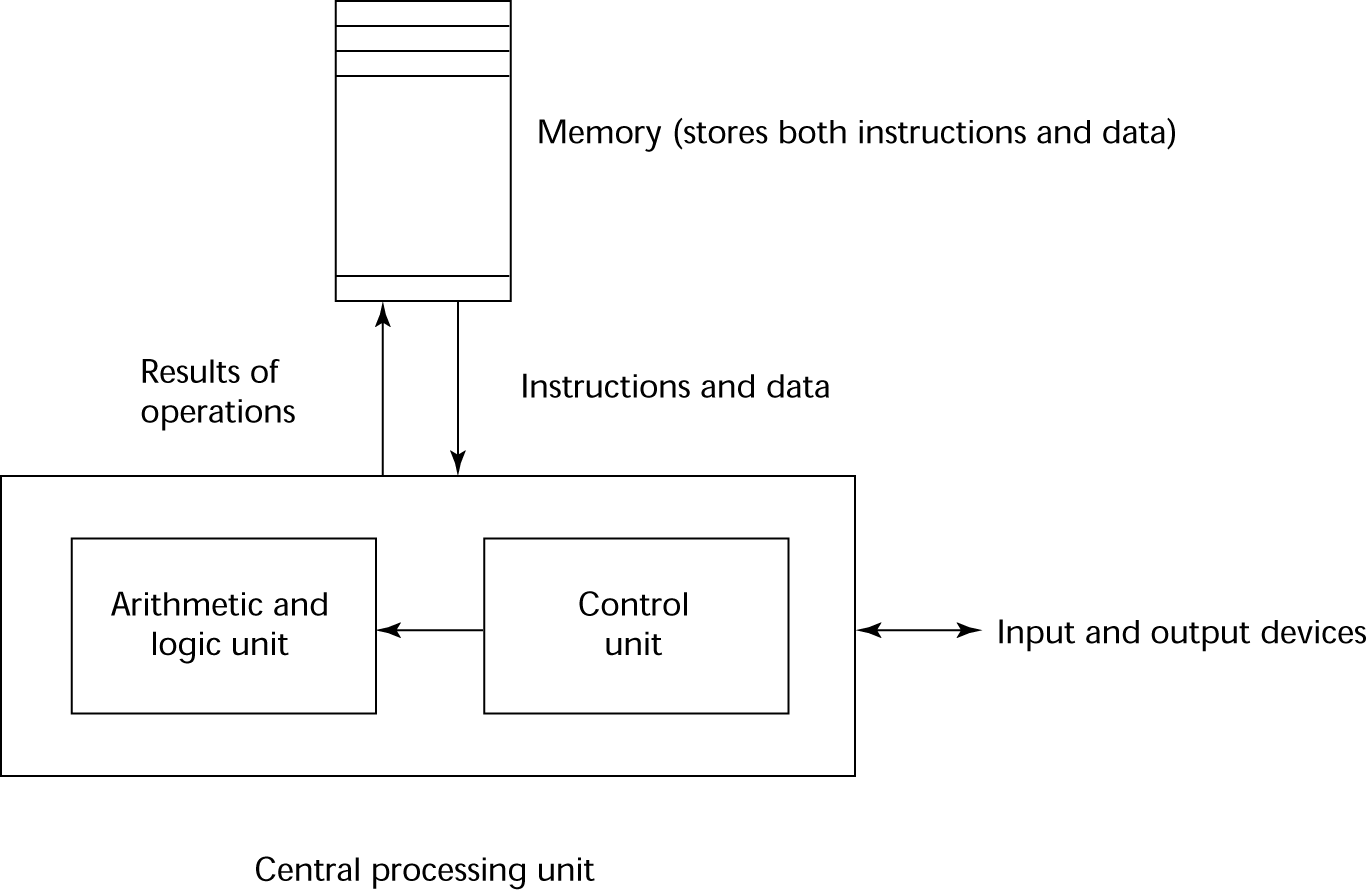
\includegraphics[width=\textwidth]{img/von_neumann.png}
		\caption{Architettura di Von Neumann.}
	\end{figure}

	\noindent
	Per operare su tali macchine, fu necessario inserire una CPU per eseguire algoritmi e operare sui dati in memoria. Il primo linguaggio che consente di programmare tale architettura è quello basato sull'implementazione dell'architettura stessa, ovvero la programmazione con schede perforate per esempio.\newpage
	
	\subsection{Definizioni}
	
	\subsubsection{Algoritmo}
	
	Un \textcolor{Red3}{\textbf{algoritmo}} \textbf{è una sequenza finita di passi primitivi di calcolo descritti mediante una frase ben formata (programma) in un linguaggio di programmazione}. In altre parole, un algoritmo scompone un calcolo complesso in passi elementari di computazione. Esso è dunque un concetto astratto che trova la sua forma concreta in un programma che è la sequenza finita di istruzioni.\newline
	
	\noindent
	Data la definizione, è necessario precisare che:
	\begin{itemize}
		\item \textbf{Un programma non è necessariamente un algoritmo}, poiché una frase grammaticalmente corretta potrebbe non avere significato;
		\item \textbf{Lo stesso algoritmo può avere concretizzazioni diverse}, ovvero lo stesso algoritmo può essere implementato da infiniti programmi.
	\end{itemize}

	\subsubsection{Dati}

	I programmi sono la concretizzazione degli algoritmi, i quali manipolano i \textcolor{Red3}{\textbf{dati}}. Essi sono informazioni memorizzate sia concretamente in celle di memoria, sia astrattamente in elementi che il linguaggio di programmazione può manipolare, ovvero le \textbf{variabili}.
	
	\subsubsection{Sintassi e semantica}

	La trasformazione (scrittura) di un programma in un determinato linguaggio di programmazione rappresenta la \textcolor{Red3}{\textbf{sintassi}}, mentre l'effetto della sua esecuzione e la trasformazione dei dati eseguita, costituisce la \textcolor{Red3}{\textbf{semantica}}.
	
	\subsubsection{Linguaggio matematico e logico}
	
	Il \textcolor{Red3}{\textbf{linguaggio matematico}} è una notazione rigorosa per rappresentare funzioni, ma non sempre oggetti infiniti e computazioni, cioè passi di calcolo.\newline
	
	\noindent
	Il \textcolor{Red3}{\textbf{linguaggio logico}} sono regole e assiomi che rendono possibile specificare il processo di computazione, in modo implicito, e consente di rappresentare formalmente oggetti infiniti in modo finito, ma non computazioni infinite.
	
	\subsubsection{Linguaggio di programmazione}
	
	Un \textcolor{Red3}{\textbf{linguaggio di programmazione}} consente di specificare in modo accurato esattamente le primitive del processo di computazione, con la rigorosità e la potenza della logica.\newpage
	
	\subsubsection{Programma}
	
	Un \textcolor{Red3}{\textbf{programma}} è un insieme finito di istruzioni e costrutti del linguaggio di programmazione.

	\longline
		
	\subsection{Aspetti di progettazione}
	
	\subsubsection{Leggibilità}
	
	La \textcolor{Red3}{\textbf{leggibilità}} (\emph{readability}) è la sintassi chiara, l'assenza di ambiguità, la facilità di lettura e la comprensione dei programmi.\newline
	
	\noindent
	I fattori che contribuiscono alla leggibilità sono:
	\begin{enumerate}
		\item La \textbf{semplicità di un linguaggio}, per esempio pochi ed essenziali costrutti base. Infatti, un linguaggio inizia ad essere complicato quando per poter fare la stessa cosa si possono seguire molti percorsi diversi. Un altro fattore di complicazione è l'overloading degli operatori, ovvero quando il simbolo di un operatore ha molteplici significati.
		
		\item L'\textbf{ortogonalità} della progettazione di un linguaggio. Un elemento di un programma è ortogonale se è indipendente dal contesto di utilizzo all'interno di esso. Più un programma è ortogonale, meno eccezioni alla regola esistono.
		
		\item \textbf{Presenza di strumenti per la definizione di tipi di dati e strutture dati}. Ad esempio l'uso di booleani al posto dei valori interi.
		
		\item \textbf{Struttura della sintassi}, come parole chiave significative ad esempio.
	\end{enumerate}
	
	\subsubsection{Scrivibilità}
	
	La \textcolor{Red3}{\textbf{scrivibilità}} (\emph{writability}) è la facilita di utilizzo di un linguaggio per creare programmi, la facilità di analisi e la verifica dei programmi. I fattori che influenza la leggibilità sono gli stessi della scrivibilità.\newline
	
	\noindent
	In breve i fattori che che contribuiscono alla scrivibilità sono:
	\begin{enumerate}
		\item \textbf{Semplicità e ortogonalità}. La presenza di pochi costrutti consente al programmatore di conoscerli in gran parte e di sfruttare al massimo il linguaggio. Stessa cosa per il numero di primitive.
		
		\item \textbf{Supporto per l'astrazione}. La possibilità di utilizzare strutture o operazioni complesse in modi che permettono di ignorare i dettagli. Esistono due tipi di astrazione: processi e dati.
		
		\item \textbf{Espressività}. Si riferisce a molte caratteristiche, per esempio mettere a disposizione un insieme di modi relativamente convenienti per specificare operazioni.
	\end{enumerate}\newpage
	
	\subsubsection{Affidabilità e costo}
	
	Per \textcolor{Red3}{\textbf{affidabilità}} (\emph{reliability}) si intende la conformità alle sue specifiche. Mentre per \textcolor{Red3}{\textbf{costo}}, letteralmente il costo complessivo di utilizzo.\newline
	
	\noindent
	Un \textbf{programma} viene categorizzato come \textbf{affidabile} se soddisfa le seguenti condizioni:
	\begin{enumerate}
		\item \textbf{\emph{Type checking}}, ovvero il controllo degli errori di tipo. Viene eseguito spesso a tempo di compilazione poiché risulta costoso.
		
		\item \textbf{Gestione delle eccezzioni}. Gestire gli errori run-time per consentire la continuazione dell'esecuzione e l'attuazione di eventuali misure correttive.
		
		\item \textbf{Presenza di potenziali aliasing}. La presenza di due o più metodi di riferimento per la stessa locazione di memoria è un problema.
	\end{enumerate}

	\noindent
	Mentre le \textbf{specifiche di costo} riguardano:
	\begin{itemize}
		\item L'addestramento di programmatore per usare il linguaggio
		\item Scrittura di programma
		\item Compilazione dei programmi
		\item Esecuzione dei programmi
		\item Sistema di implementazione del linguaggio, ovvero la disponibilità di compilatori liberi
		\item Poca affidabilità fanno lievitare i costi
		\item Mantenimento dei programmi
	\end{itemize}\newpage

	\subsection{Classificazione dei linguaggi}
	
	I linguaggi possono essere classificati per: \textbf{metodo di computazione} e \textbf{per caratteristiche}.
	
	\subsubsection{Metodo di computazione}
	
	I linguaggi possono essere a:
	\begin{itemize}
		\item \textcolor{Red3}{\textbf{Basso livello}}. Questi linguaggi hanno caratteristiche strettamente dipendente all'architettura su cui si sta programmando. Per esempio:
		\begin{itemize}
			\item Linguaggio binario che non fa distinzione tra dati e programmi;

			\item Assembly, linguaggio strutturato molto basso, vicino al linguaggio macchina.
		\end{itemize}
	
		\item \textcolor{Red3}{\textbf{Alto livello}}. Questi linguaggi consentono una programmazione strutturata in cui dati ed istruzioni hanno rappresentazioni diverse. Esistono tre tipi:
		\begin{itemize}
			\item \textcolor{Red3}{\textbf{Linguaggi imperativi}} che descrivono come \textbf{concetto chiave} l'elemento fondamentale dell'architettura di Von Neumann, ovvero la \textbf{cella di memoria}.\newline
			Il concetto di variabile rappresenta l'astrazione logica della cella.\newline
			Il concetto di assegnamento rappresenta l'operazione primitiva di modifica della cella di memoria e dunque dello stato della macchina.\newline
			Nei linguaggi imperativi, gli assegnamenti vengono controllati in modo sequenziale, condizionale e ripetuti.
			
			\item \textcolor{Red3}{\textbf{Linguaggi funzionali}} sono molto vicini alla matematica. Essi descrivono i passi di calcolo come funzioni matematiche. Il \emph{core} principale si concentra sulla composizione e applicazione di funzioni.\newline
			Una variabile viene intesa come un'incognita matematica e sostituita come se fosse un \emph{placeholder} all'interno del linguaggio. Infatti, essa \underline{non} può cambiare nel tempo durante la computazione.
			
			\item \textcolor{Red3}{\textbf{Linguaggi logici}} usano la logica, ovvero eseguono pattern matching. Come passo di calcolo primitivo utilizzano l'unificazione o la sostituzione.
		\end{itemize}
	\end{itemize}

	\subsubsection{Per caratteristiche}
	
	La classificazione per caratteristiche è una metodologia utilizzata principalmente all'inizio dell'era informatica per studiare le caratteristiche di base quali: strutture di base di controllo, strutture per i dati, efficienze nell'esecuzione.\newline
	
	\noindent
	Andando avanti con il tempo, la classificazione si è focalizzata su caratteristiche aggiuntive, ovvero le strutture di base rimangono le stesse, ma ad esse vengono aggiunte nuove caratteristiche. In questo modo viene migliorata la soluziona di specifici problemi.\newpage
	
	\subsection{Implementazione dei linguaggi}
	
	L'\textbf{implementazione di un linguaggio} ha un collegamento stretto con il funzionamento della macchina su cui deve essere eseguito. Infatti, l'implementazione riguarda le metodologie per rendere comprensibile alla macchina da programmare il linguaggio scelto. Per farlo, è necessario introdurre il funzionamento di una macchina basata sull'architettura di Von Neumann. Essa si basa sulla ripetizione di un ciclo che costituisce l'\textbf{interprete} del linguaggio che la macchina riconosce:
	\begin{itemize}
		\item Lettura dell'istruzione dalla memoria (\emph{fetch})
		
		\item Decodifica dell'istruzione (\emph{decode})
		
		\item Lettura di eventuali operandi
		
		\item Memorizzazione ed esecuzione del risultato (\emph{exec})
	\end{itemize}
	\begin{figure}[!htp]
		\centering
		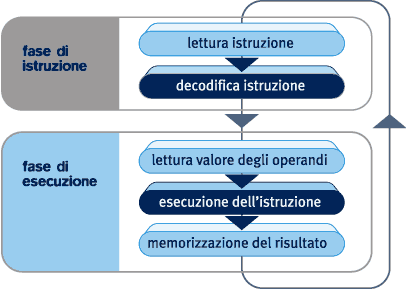
\includegraphics[width=.75\textwidth]{img/fasi_esecuzione.png}
		\caption{Ciclo di esecuzione delle istruzioni.}
	\end{figure}

	\subsubsection{Macchina astratta}

	\noindent
	L'implementazione di un linguaggio \textbf{significa} considerare una macchina astratta poiché lavorando ad alto livello, le istruzioni vengono interpretate e dunque si ignorano momentaneamente il linguaggio binario e la macchina fisica.\newline
	
	\noindent
	Dato un linguaggio $L$ di programmazione, la \textcolor{Red3}{\textbf{macchina astratta}} $M_{L}$ per $L$ è un insieme di strutture dati ed algoritmi che permettono di memorizzare ed eseguire i programmi scritti in $L$.\newpage
	
	\noindent
	La collezione di strutture dati ed algoritmi è necessario per:
	\begin{itemize}
		\item Acquisire la prossima istruzione
		
		\item Gestire le chiamate e i ritorni dai sottoprogrammi
		
		\item Acquisire gli operandi e memorizzare i risultati delle operazioni
		
		\item Mantenere le associazioni fra nomi e valori denotati
		
		\item Gestire dinamicamente la memoria
	\end{itemize}

	\noindent
	In altre parole, una \textbf{macchina astratta} è la combinazione di una memoria che immagazzina i programmi e di un interprete che esegue istruzioni dei programmi.
	\begin{figure}[!htp]
		\centering
		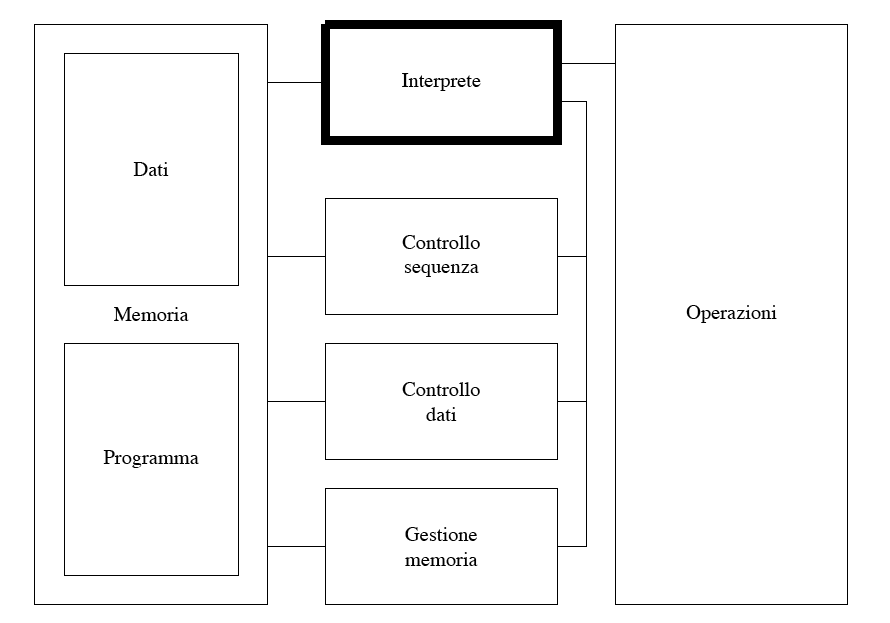
\includegraphics[width=\textwidth]{img/macchina_astratta.png}
		\caption{Rappresentazione di una macchina astratta.}
	\end{figure}
	
	\noindent
	Il \textbf{linguaggio} $L$ riconosciuto (interpretato) dalla macchina astratta $M_{L}$ viene chiamato \textbf{linguaggio macchina}. Formalmente, è l'insieme di tutte le stringhe interpretabili dalla macchina astratta $M$.\newpage
	
	\subsubsection{Realizzazione di una macchina astratta a vari livelli}
	
	Qualsiasi macchina astratta, per essere eseguita, deve prima o poi utilizzare qualche dispositivo hardware. Questo però non significa che tutte le macchine sono realizzate a livello hardware. Infatti, la realizzazione di una macchina astratta può avvenire tre categorie:
	\begin{itemize}
		\item \textcolor{Red3}{\textbf{Realizzazione hardware (HW)}}. Sempre possibile e concettualmente semplice. Il linguaggio macchina è il linguaggio fisico/binario e si realizza mediante dispositivi fisici. Data la sua lontananza dai linguaggi ad alto livello, la loro programmazione risulta complessa. Questo è uno dei tanti motivi per cui viene usata solo per sistemi dedicati.
		
		\item \textcolor{Red3}{\textbf{Realizzazione firmware (FW)}}. Le strutture dati e gli algoritmi vengono simulati nella macchina mediante microprogrammi. Il linguaggio macchina è a basso livello e consiste in microistruzioni che specificano le operazioni di trasferimento dati tra registri. Il vantaggio è dato dalla velocità e la flessibilità maggiore rispetto all'hardware.
		
		\item \textcolor{Red3}{\textbf{Realizzazione software (SW)}}. Le strutture dati e gli algoritmi vengono realizzati tramite un linguaggio implementato. In questo modo è possibile scrivere programmi che interpretano i costrutti del linguaggio macchina simulando le funzionalità della macchina. La velocità viene diminuita ma aumenta molto la flessibilità.
	\end{itemize}\newpage

	\subsubsection{Realizzazione software e livelli di astrazione}
	
	Con la realizzazione software, vengono utilizzati linguaggi di programmazione ad alto livello poiché essi implementano una struttura suddivisa a livelli di astrazione. Ogni livello coopera in modo sequenziale ma allo stesso tempo è indipendente.
	
	\begin{figure}[!htp]
		\centering
		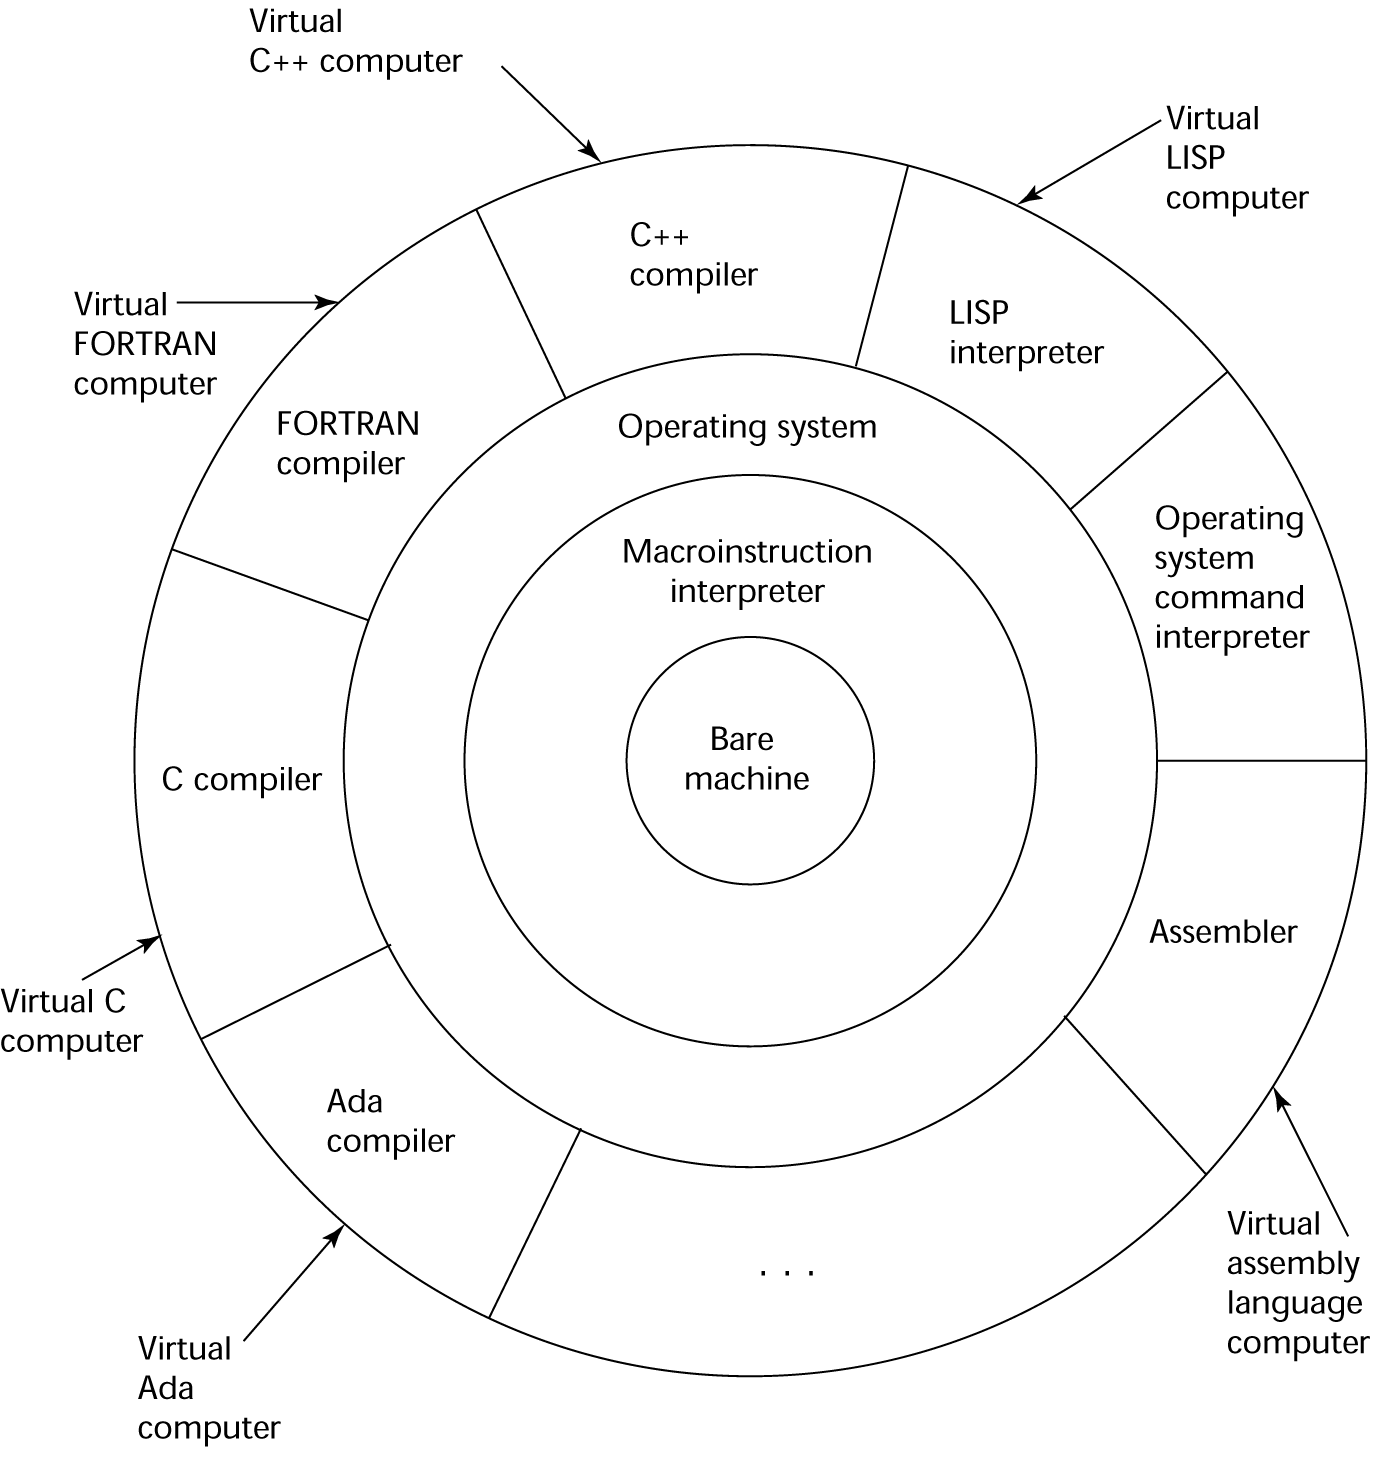
\includegraphics[width=.8\textwidth]{img/astrazione.png}
		\caption{Livelli di astrazione utilizzati dai linguaggi ad alto livello.}
	\end{figure}

	\noindent
	Quindi, la macchina può essere vista come una stratificazione di livelli di astrazione:
	\begin{figure}[!htp]
		\centering
		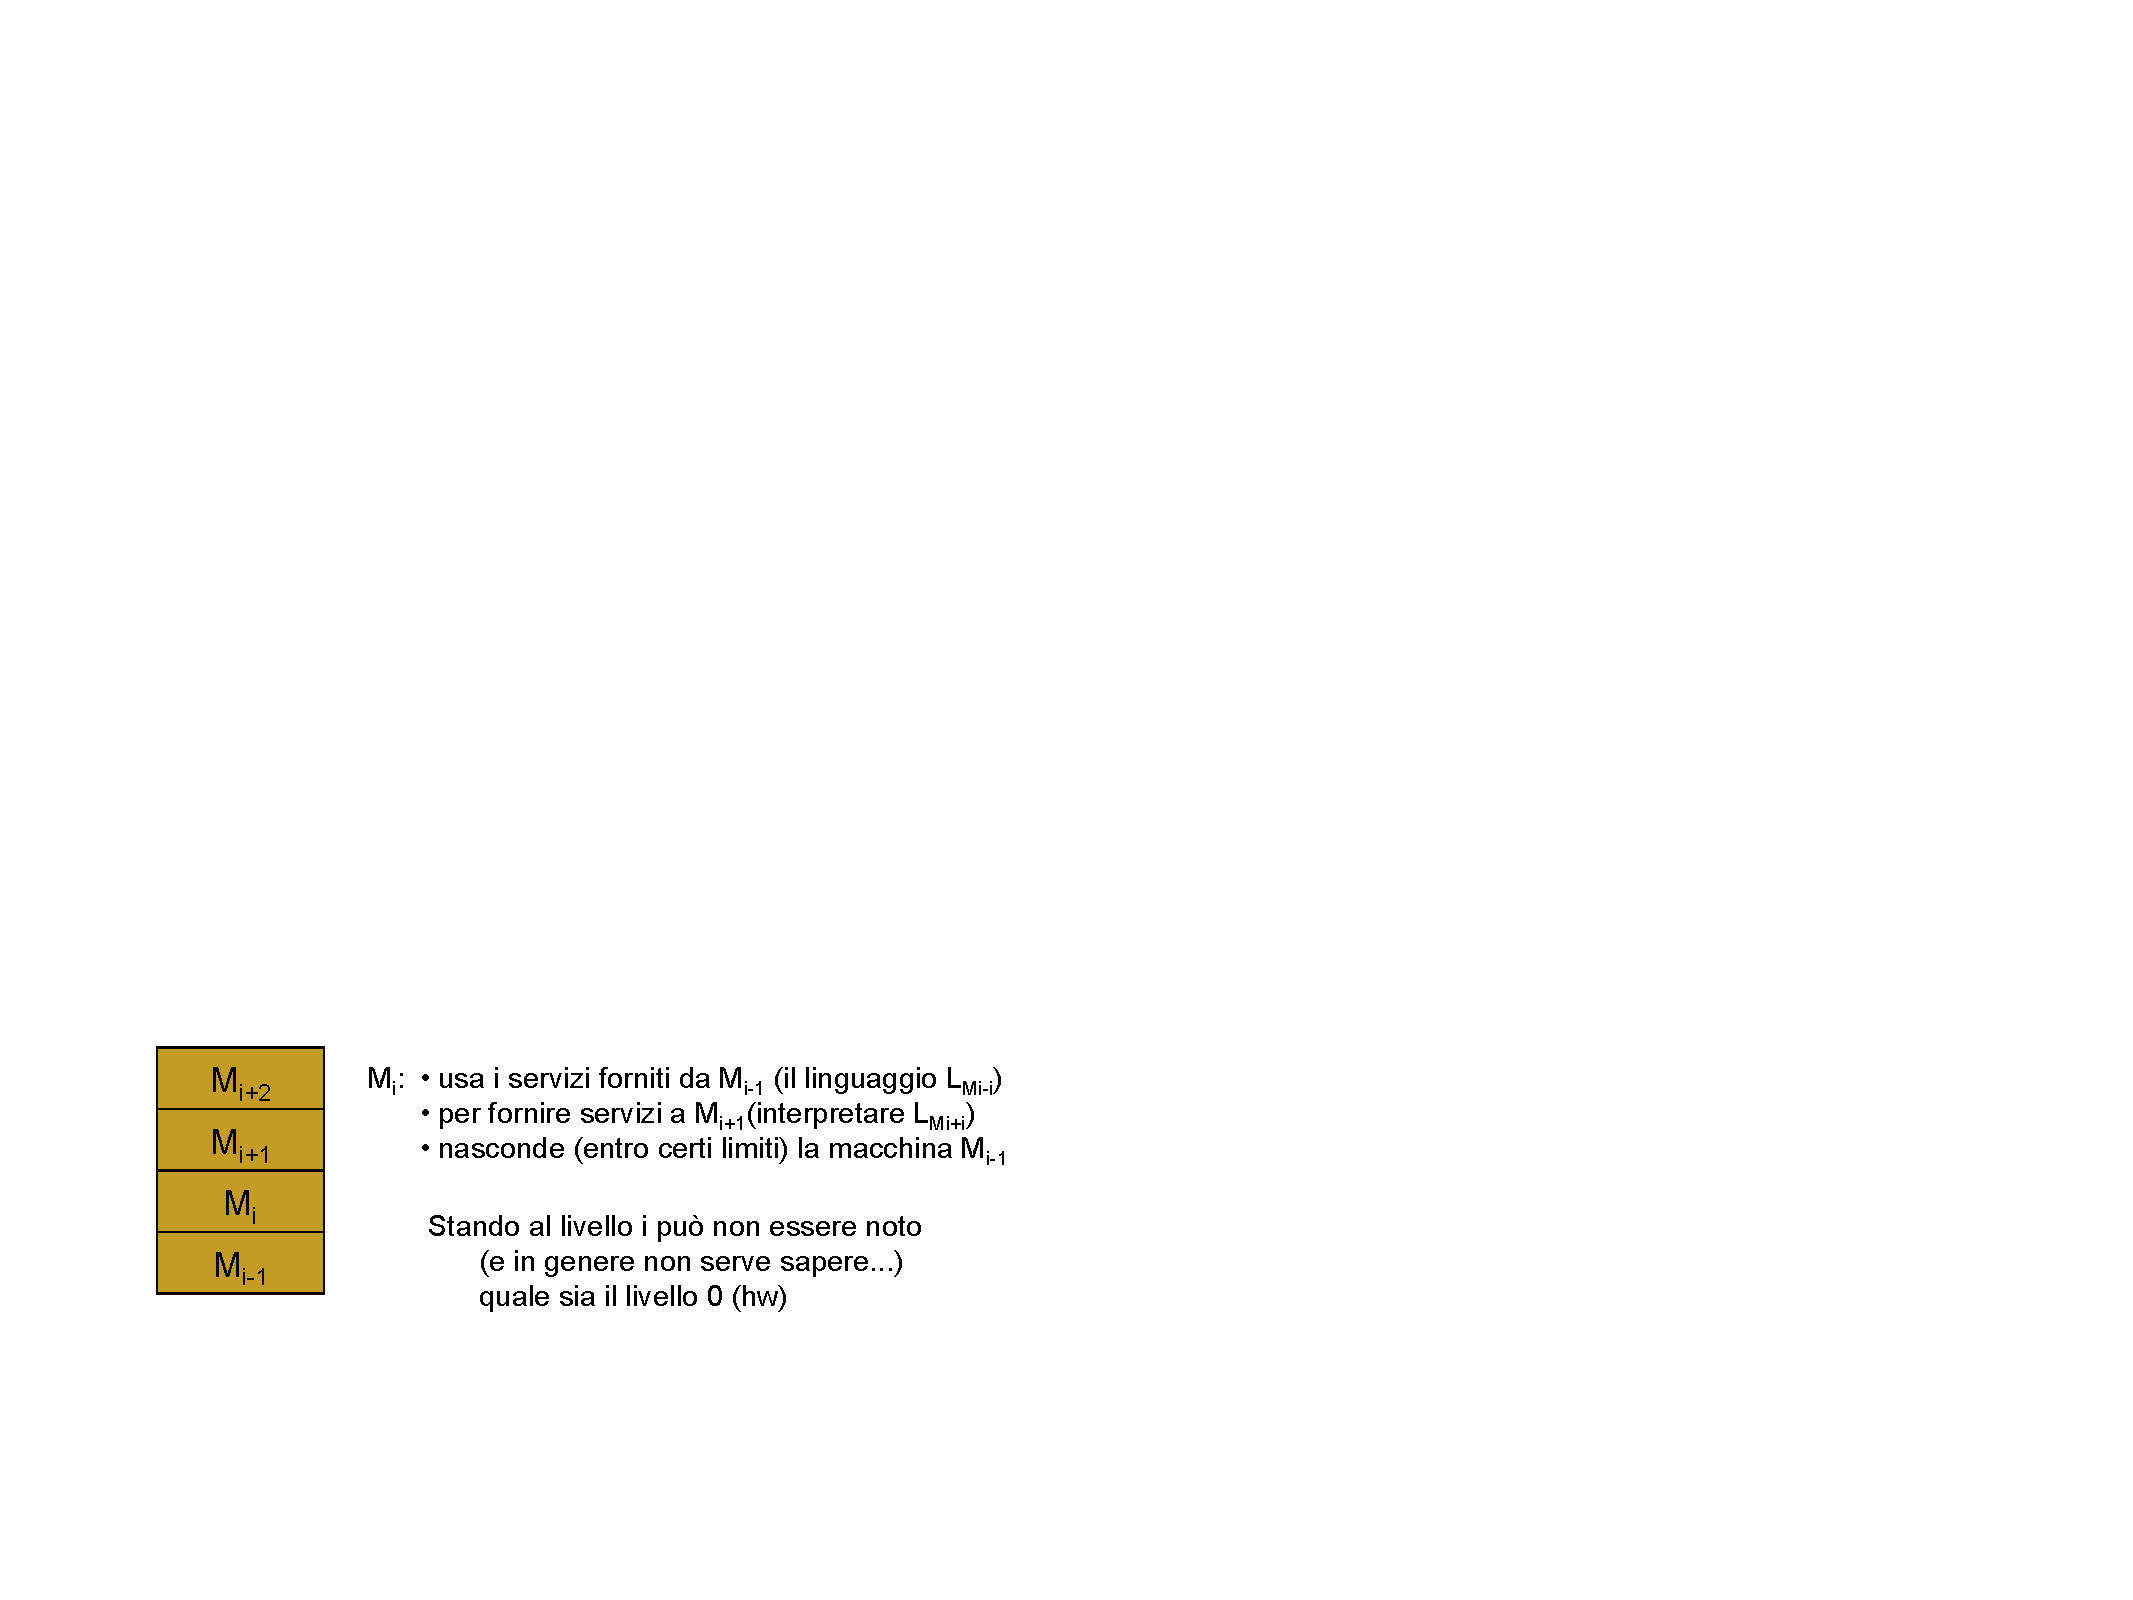
\includegraphics[width=.8\textwidth]{img/livelli_astrazione_macchina.pdf}
	\end{figure}\newpage

	\subsection{Realizzazione di una macchina a livello software/firmware}
	
	Sia $L$ un linguaggio da implementare e sia $M_{L_{0}}$ una macchina astratta a disposizione che ha come linguaggio macchina $L_{0}$. La macchina astratta $M_{L_{0}}$ è il livello su cui si vuole implementare il linguaggio $L$ e che mettette a disposizione di $M_{L}$ le sue funzionalità.\newline
	
	\noindent
	Dunque, la realizzazione di una macchina astratta $M_{L}$ consiste nel realizzare una macchina che \dquotes{traduce} il linguaggio $L$ (ad alto livello per esempio) in linguaggio macchina $L_{0}$, ovvero che interpreta tutte le istruzioni di $L$ come istruzioni di $L_{0}$. La traduzione avviene tramite due metodi a scelta:
	\begin{itemize}
		\item \textbf{Soluzione interpretativa}. Simulazione dei costrutti della macchina astratta $M_{L}$ da realizzare, mediante programmi scritti in $L_{0}$;
		\item \textbf{Soluzione compilativa}. Traduzione esplicita dei programmi di $L$ in corrispondenti programmi di $L_{0}$.
	\end{itemize}\newpage

	\subsubsection{Soluzione interpretativa: interprete}\label{interprete}
	
	La soluzione interpretativa prevede l'utilizzo di un interprete per la realizzazione di una macchina astratta. Un \textcolor{Red3}{\textbf{interprete}} è un programma $\mathrm{int}^{\mathrm{L_{0}, L}}$ che esegue, sulla macchina astratta per $L_{0}$, programmi $P^{L}$, scritti nel linguaggio di programmazione $L$, su un input fissato appartenente all'insieme di dati (input e output). In breve, un interprete è una \textbf{macchina universale} che preso un programma e un suo input, lo esegue su quell'input usando solo funzionalità messe a disposizione dal livello (macchina astratta) sottostante.
	\begin{center}
		\textcolor{Red3}{\textbf{\emph{Notazioni}}}
	\end{center}
	\begin{itemize}
		\item $Prog^{L}$ è l'insieme di programmi scritti nel linguaggio di programmazione $L$;
		\item $D$ è l'insieme di dati, ovvero input e output;
		\item $P^{L}$ è il programma scritto nel linguaggio di programmazione $L$;
		\item Relazioni ovvie: $P^{L} \in Prog^{L}$ e $in, out \in D$;
		\item $\exec{P^{L}}: D \longrightarrow D$ è la notazione utilizzata per indicare che l'esecuzione del programma scritto nel linguaggio di programmazione $L$ con input $in$ è uguale all'output $out$. Quindi $\exec{P^{L}}\left(in\right) = out$.
	\end{itemize}
	Un \textcolor{Red3}{\textbf{interprete formalmente}} (\textbf{definizione}) è esprimibile nel seguente modo. Si consideri un interprete da $L$ a $L_{0}$: dato $P^{L} \in Prog^{L}$ e $in \in D$, un interprete $int^{L, L_{0}}$ per $L$ su $L_{0}$ è un programma tale che $\exec{int^{L, L_{0}}}: \left(Prog^{L}\right) \longrightarrow D$ e dunque $\exec{int^{L, L_{0}}}\left(P^{L}, in\right) = \exec{P^{L}}\left(in\right)$.\newline
	
	\noindent
	Anche un programma può essere utilizzato come dato di input in un altro programma. Si osservi il seguente diagramma:
	\begin{figure}[!htp]
		\centering
		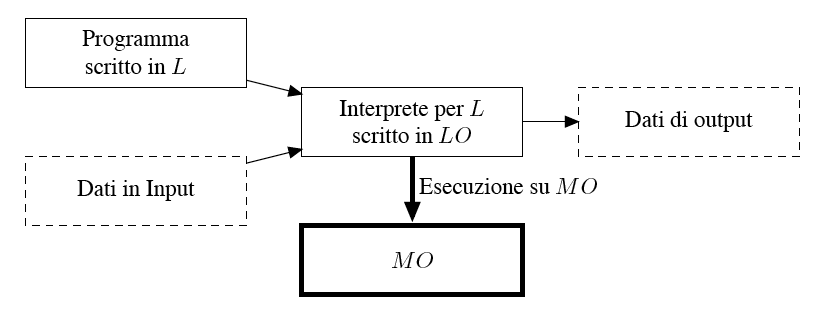
\includegraphics[width=\textwidth]{img/programma_input.png}
	\end{figure}
	
	\noindent
	Si noti come un programma scritto nel linguaggio $L$, insieme ad eventuali altri input, viene interpretato da un programma creato appositamente per eseguire questo compito su $L$, ma scritto in $L_{0}$. L'\textbf{esecuzione comporta una decodifica e non una traduzione esplicita}. Infatti, l'interprete simula ogni istruzione di $L$ utilizzando un certo insieme di istruzioni di $L_{0}$. Questa è la base dei linguaggi di scripting.
	
	\subsubsection{Soluzione interpretativa: operazioni e struttura}
	
	Un interprete può eseguire una serie di \textbf{operazioni}:
	\begin{itemize}
		\item \textcolor{Red3}{\textbf{Elaborazione dei dati primitivi}}. I dati primitivi sono dati rappresentabili in modo diretto nella memoria, per esempio i numeri. Le elaborazioni di essi, sono implementate direttamente nella struttura della macchina;
		
		\item \textcolor{Red3}{\textbf{Controllo di sequenza delle esecuzioni}}. Non è altro che la gestione del flusso di esecuzione delle istruzioni, le quali non sempre sono sequenziali, tramite alcune strutture dati;
		
		\item \textcolor{Red3}{\textbf{Controllo dei dati}}. Recupero dei dati necessari per eseguire le istruzioni. I dati possono riguardare le modalità di indirizzamento della memoria e l'ordine con cui recuperare gli operandi;
		
		\item \textcolor{Red3}{\textbf{Controllo della memoria}}. È necessaria una gestione della memoria per allocare dati e programmi. Cambia a seconda del tipo di realizzazione della macchina astratta:
		\begin{itemize}
			\item Realizzazione hardware (HW): la gestione è semplice poiché nella peggiore delle ipotesi, i dati potrebbero essere rimasti sempre nelle stesse locazioni.
			
			\item Realizzazione software (SW): la gestione è complessa ed esistono costrutti di allocazione e deallocazione che richiedono alcune strutture dati (e.g. pile) e operazioni dinamiche.
		\end{itemize}
	\end{itemize}
	Date le operazioni elencate, il \textcolor{Red3}{\textbf{ciclo di esecuzione di un interprete}} è il seguente:
	\begin{lstlisting}[language=C]
begin
	go := true;
	while go do begin
		FETCH(OPCODE, OPINFO) at PC
		DECODE(OPCODE, OPINFO)
		if OPCODE needs ARGS then FETCH (ARGS)
		case OPCODE of
			OP1: EXECUTE(OP1, ARGS)
			...
			OPn: EXECUTE(OPn, ARGS)
			HLT: go := false;
		if OPCODE has result then STORE(RES);
		PC := PC + SIZE(OPCODE);
	end
end \end{lstlisting}
	\begin{itemize}
		\item Righe 1-3: finché \textsf{go} ha il valore \textsf{true}, il codice viene eseguito;
		\item Riga 4: estrazione dell'istruzione riferita ad \textsf{OPCODE} (controllo sequenza 1 su 2);
		\item Righe 5: decodifica dell'istruzione estratta alla riga precedente;
		\item Riga 6: prelievo dalla memoria gli operandi richiesti da \textsf{OPCODE} e nelle modalità individuate (controllo dati 1 su 2);
		\item Righe 7-11: esecuzione delle operazioni;
		\item Riga 12: se l'operazione ha un risultato da salvare, allora viene salvato in memoria (controllo dati 2 su 2);
		\item Riga 13: viene incrementato il \emph{program counter} (PC) per eseguire la prossima istruzione (controllo sequenza 2 su 2).
	\end{itemize}
	Il ciclo continua ad essere eseguito finché la variabile \textsf{go} ha valore \textsf{true}. Inoltre, le istruzioni riferite al program counter sono chiamate istruzioni di \textbf{controllo sequenza} (CS) perché manipolano e accedono al program counter. Mentre le operazioni di memorizzazione/estrazione sugli argomenti si chiamano \textbf{controllo dati} (CD).
	\begin{figure}[!htp]
		\centering
		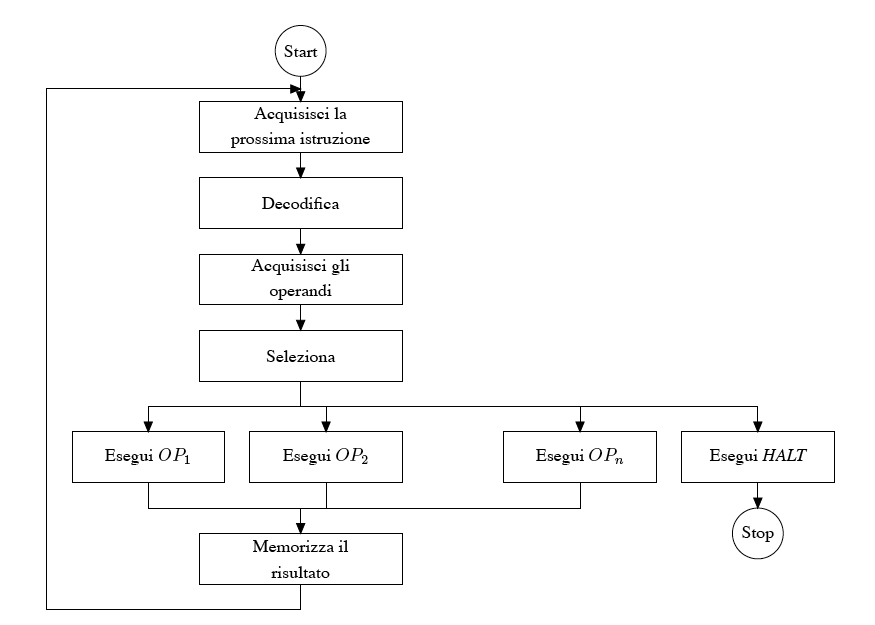
\includegraphics[width=\textwidth]{img/ciclo_esecuzione_interprete.png}
		\caption{Diagramma a blocchi della struttura di un interprete.}
	\end{figure}\newpage

	\subsubsection{Soluzione interpretativa: pro e contro}
	
	\begin{itemize}
		\item \textcolor{Green4}{\textbf{Pro:}}
		\begin{itemize}
			\item \textbf{Facilità di interazione \emph{run-time}}. Interpretazione al momento dell'esecuzione consente di interagire direttamente con l'esecuzione del programma (\emph{debugging});
			\item Velocità nello sviluppo applicativo di un interprete, quindi \textbf{tempi ridotti per la sua creazione};
			\item Utilizzo della \textbf{memoria ridotto} rispetto ad un compilatore.
		\end{itemize}

		\item \textcolor{Red3}{\textbf{Contro:}}
		\begin{itemize}
			\item Tempi di decodifica sommati a quelli d'esecuzione ogni volta che un'istruzione viene eseguita, si traduce in un'\textbf{esecuzione lenta} e quindi una scarsa efficienza della macchina.
		\end{itemize}
	\end{itemize}\newpage
	
	\subsubsection{Soluzione compilativa: compilatore}\label{compilatore}

	Un \textcolor{Red3}{\textbf{compilatore}} è un programma $\mathrm{comp}^{L_{0}, L}$ che \textbf{traduce}, preservando semantica e funzionalità, programmi scritti nel linguaggio di programmazione $L$ in programmi scritti in $L_{0}$, e quindi eseguibili direttamente sulla macchina astratta per $L_{0}$.
	Come l'interprete, anche il compilatore accetta un programma come input poiché viene considerato come dato.
	\begin{center}
		\textcolor{Red3}{\textbf{\emph{Notazioni}}}
	\end{center}
	\begin{itemize}
		\item $Prog^{L}$ è l'insieme di programmi scritti nel linguaggio di programmazione $L$;
		\item $D$ è l'insieme di dati, ovvero input e output;
		\item $P^{L}$ è il programma scritto nel linguaggio di programmazione $L$;
		\item Relazioni ovvie: $P^{L} \in Prog^{L}$ e $in, out \in D$;
		\item $\exec{P^{L}}: D \longrightarrow D$ rappresenta la semantica di $P^{L}$.
	\end{itemize}
	Un \textcolor{Red3}{\textbf{compilatore formalmente}} (\textbf{definizione}) è esprimibile nel seguente modo.\newline
	Dato $P^{L} \in Prog^{L}$, un \textbf{compilatore} $\mathrm{comp}^{L, L_{0}}$ da $L$ a $L_{0}$ è un programma tale che $\exec{comp^{L, L_{0}}}: Progr^{L} \longrightarrow Progr^{L_{0}}$ e:
	\begin{equation*}
		\exec{comp^{L, L_{0}}}\left(P^{L}\right) = P^{L_{0}} \text{ tale che } \forall in \in D. \exec{P^{L_{0}}}\left(in\right) = \exec{P^{L}}\left(in\right)
	\end{equation*}
	Ovvero che l'esecuzione della compilazione del linguaggio $L$ a $L_{0}$ con input il programma scritto in $L$, l'output sia uguale al programma scritto nel linguaggio $L_{0}$; tale che per ogni input appartenente all'insieme dei dati, l'esecuzione del programma scritto in $L_{0}$ con input $in$, sia uguale all'esecuzione del programma scritto in $L$ con input $in$.\newline

	\noindent
	Con un compilatore, la \textbf{traduzione} è \textbf{esplicita} poiché il codice in $L$ viene prodotto come output e non eseguito. Quindi, per eseguire il programma $P^{L}$ con input $in$, è necessario prima eseguire $comp^{L, L_{0}}$ con $P^{L}$ come input.
	L'esecuzione avverrà sulla macchina astratta $M_{A}$ del linguaggio in cui è scritto il compilatore. Il risultato dunque è un altro programma (compilato) $P^{L_{0}}$, scritto in $L_{0}$. Solo a questo punto è possibile eseguire $P^{L_{0}}$ su $M_{L_{0}}$ con input $in$.
	Un \textbf{esempio} di linguaggio compilato è il C.
	\begin{figure}[!htp]
		\centering
		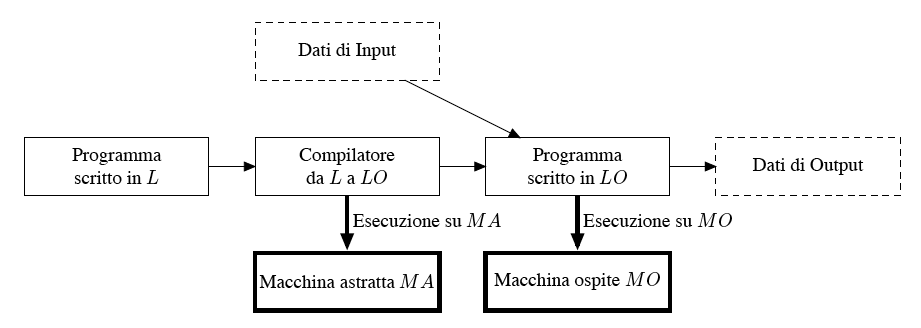
\includegraphics[width=\textwidth]{img/compilatore.png}
	\end{figure}\newpage

	\subsubsection{Soluzione compilativa: struttura}

	La compilazione deve tradurre un programma da un linguaggio ad un altro preservandone la semantica: si deve avere la certezza che il programma compilato faccia esattamente quello che faceva il sorgente. L'\textcolor{Red3}{\textbf{esecuzione}} di un compilatore si articola in varie fasi:
	\begin{figure}[!htp]
		\centering
		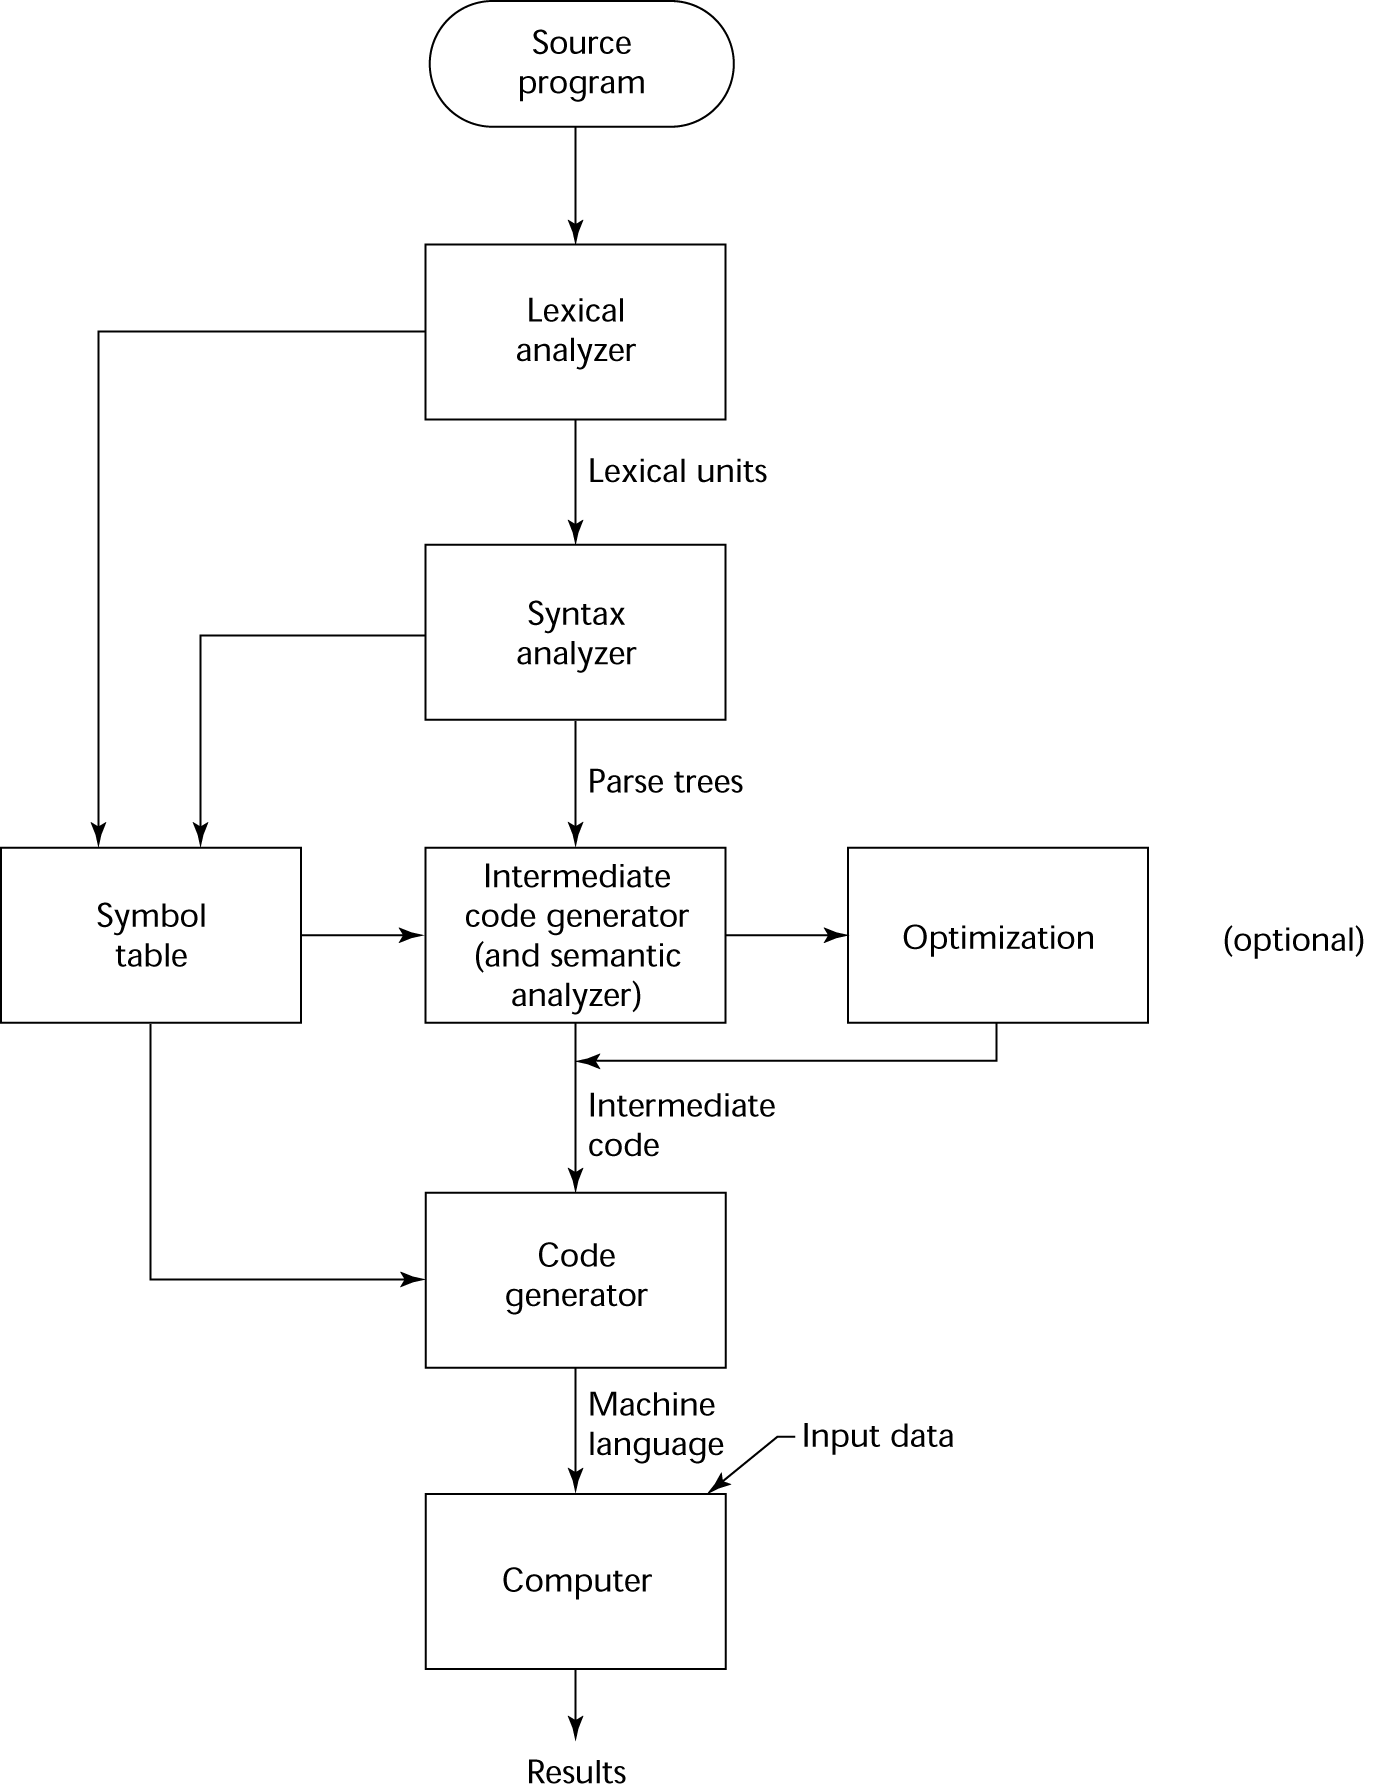
\includegraphics[width=.85\textwidth]{img/fasi_compilatore.png}
	\end{figure}
	
	\begin{itemize}
		\item \textcolor{Red3}{\textbf{Analisi lessicale}} (\emph{Lexical analyzer}), divide il programma in componenti sintattici primitivi chiamati \textbf{tokens} (identificatori, numeri, parole riservate). I \emph{tokens} sono coloro che formano i linguaggi regolari.\newline
		In altre parole, l'\textbf{analisi lessicale converte caratteri del programma sorgente in unità lessicali};\newpage

		\item \textcolor{Red3}{\textbf{Analisi sintattica}} (\emph{Syntax analyzer}), crea una rappresentazione ad albero della sintassi del programma. Ogni foglia è un \emph{token} e le foglie lette da sinistra verso destra costituiscono frasi ben formate del linguaggio. Inoltre, l'albero costituisce la struttura logica del programma e dunque nel momento in cui non fosse possibile costruire l'albero, significherebbe che qualche frase è illegale. Questo genere di evento si traduce in un errore di compilazione. Le frasi di token formano linguaggi CF.\newline
		In altre parole, l'\textbf{analisi sintattica trasforma unità lessicali in \emph{parse tree} che rappresentano la struttura sintattica del programma}.

		\item \textcolor{Red3}{\textbf{Tabella dei simboli}} (\emph{Symbol table}), memorizza le informazioni sui nomi presente nel programma, come gli identificatori, le chiamate di procedura, ecc.
		
		\item \textcolor{Red3}{\textbf{Analisi semantica}} (\emph{Semantic analyzer}), consente di rilevare errori semantici, grazie all'analisi semantica, e di generare codice intermedio che ha la caratteristica di essere indipendente dall'architettura (compito del \emph{Intermediate code generator}).

		\item \textcolor{Red3}{\textbf{Ottimizzazione}} (\emph{Optimization}), opzionale, consente di ottimizzare il codice.

		\item \textcolor{Red3}{\textbf{Generatore di codice}} (\emph{Code generator}), viene generato codice macchina che ha la caratteristica di essere dipendente dall'architettura.
	\end{itemize}

	\longline

	\subsubsection{Soluzione compilativa: pro e contro}
	
	\begin{itemize}
		\item \textcolor{Green4}{\textbf{Pro:}}
		\begin{itemize}
			\item \textbf{Esecuzione molto efficiente}, il codice viene anche ottimizzato;
		\end{itemize}

		\item \textcolor{Red3}{\textbf{Contro:}}
		\begin{itemize}
			\item \textbf{Interazione \emph{run-time} molto difficile};
			\item Un \textbf{errore} a \emph{run-time} è \textbf{difficile da associare} all'esatto comando del codice sorgente (debugging complesso);
		\end{itemize}
	\end{itemize}\newpage

	\subsubsection{Soluzione reale: ibrido}\label{ibrido}

	Nella realtà esiste un compromesso tra compilatore e interprete. Ovvero, una \textcolor{Red3}{\textbf{soluzione ibrida}} dove il linguaggio
	ad alto livello viene compilato in un linguaggio a più basso livello che poi viene interpretato.
	\begin{figure}[!htp]
		\centering
		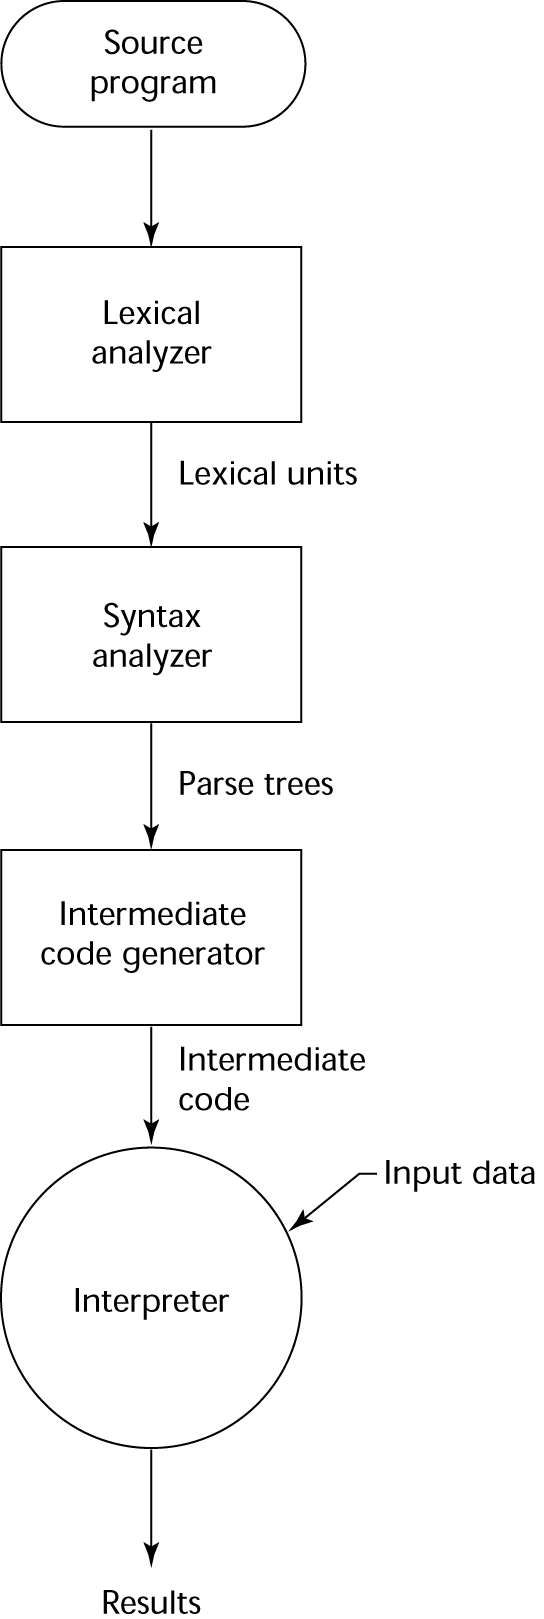
\includegraphics[width=.3\textwidth]{img/soluzione_reale_ibrida.png}
	\end{figure}

	\noindent
	Il \textbf{procedimento} è il seguente.\newline
	Si consideri il linguaggio ad alto livello $L$ per il quale si deve realizzare la macchina astratta $M_{L}$.\newline
	Il linguaggio $L$ viene quindi tradotto in un linguaggio intermedio $L_{Mi}$ la cui macchina astratta $M_{I}$ consiste in un interprete del linguaggio $L_{Mi}$ sulla macchina ospite $M_{O}$.\newline

	\noindent
	La separazione non è netta poiché vengono interpretati i costrutti lontani da $M_{O}$, mentre viene compilato il resto. Il passaggio chiave è la traduzione (compilazione) da $L$ ad un linguaggio intermedio (quello interpretato). Questo accade spesso nella realtà, specialmente con le \emph{system call} del sistema operativo. In parole povere, si cerca di trovare una connessione a metà strada.\newpage
	\begin{figure}[!htp]
		\centering
		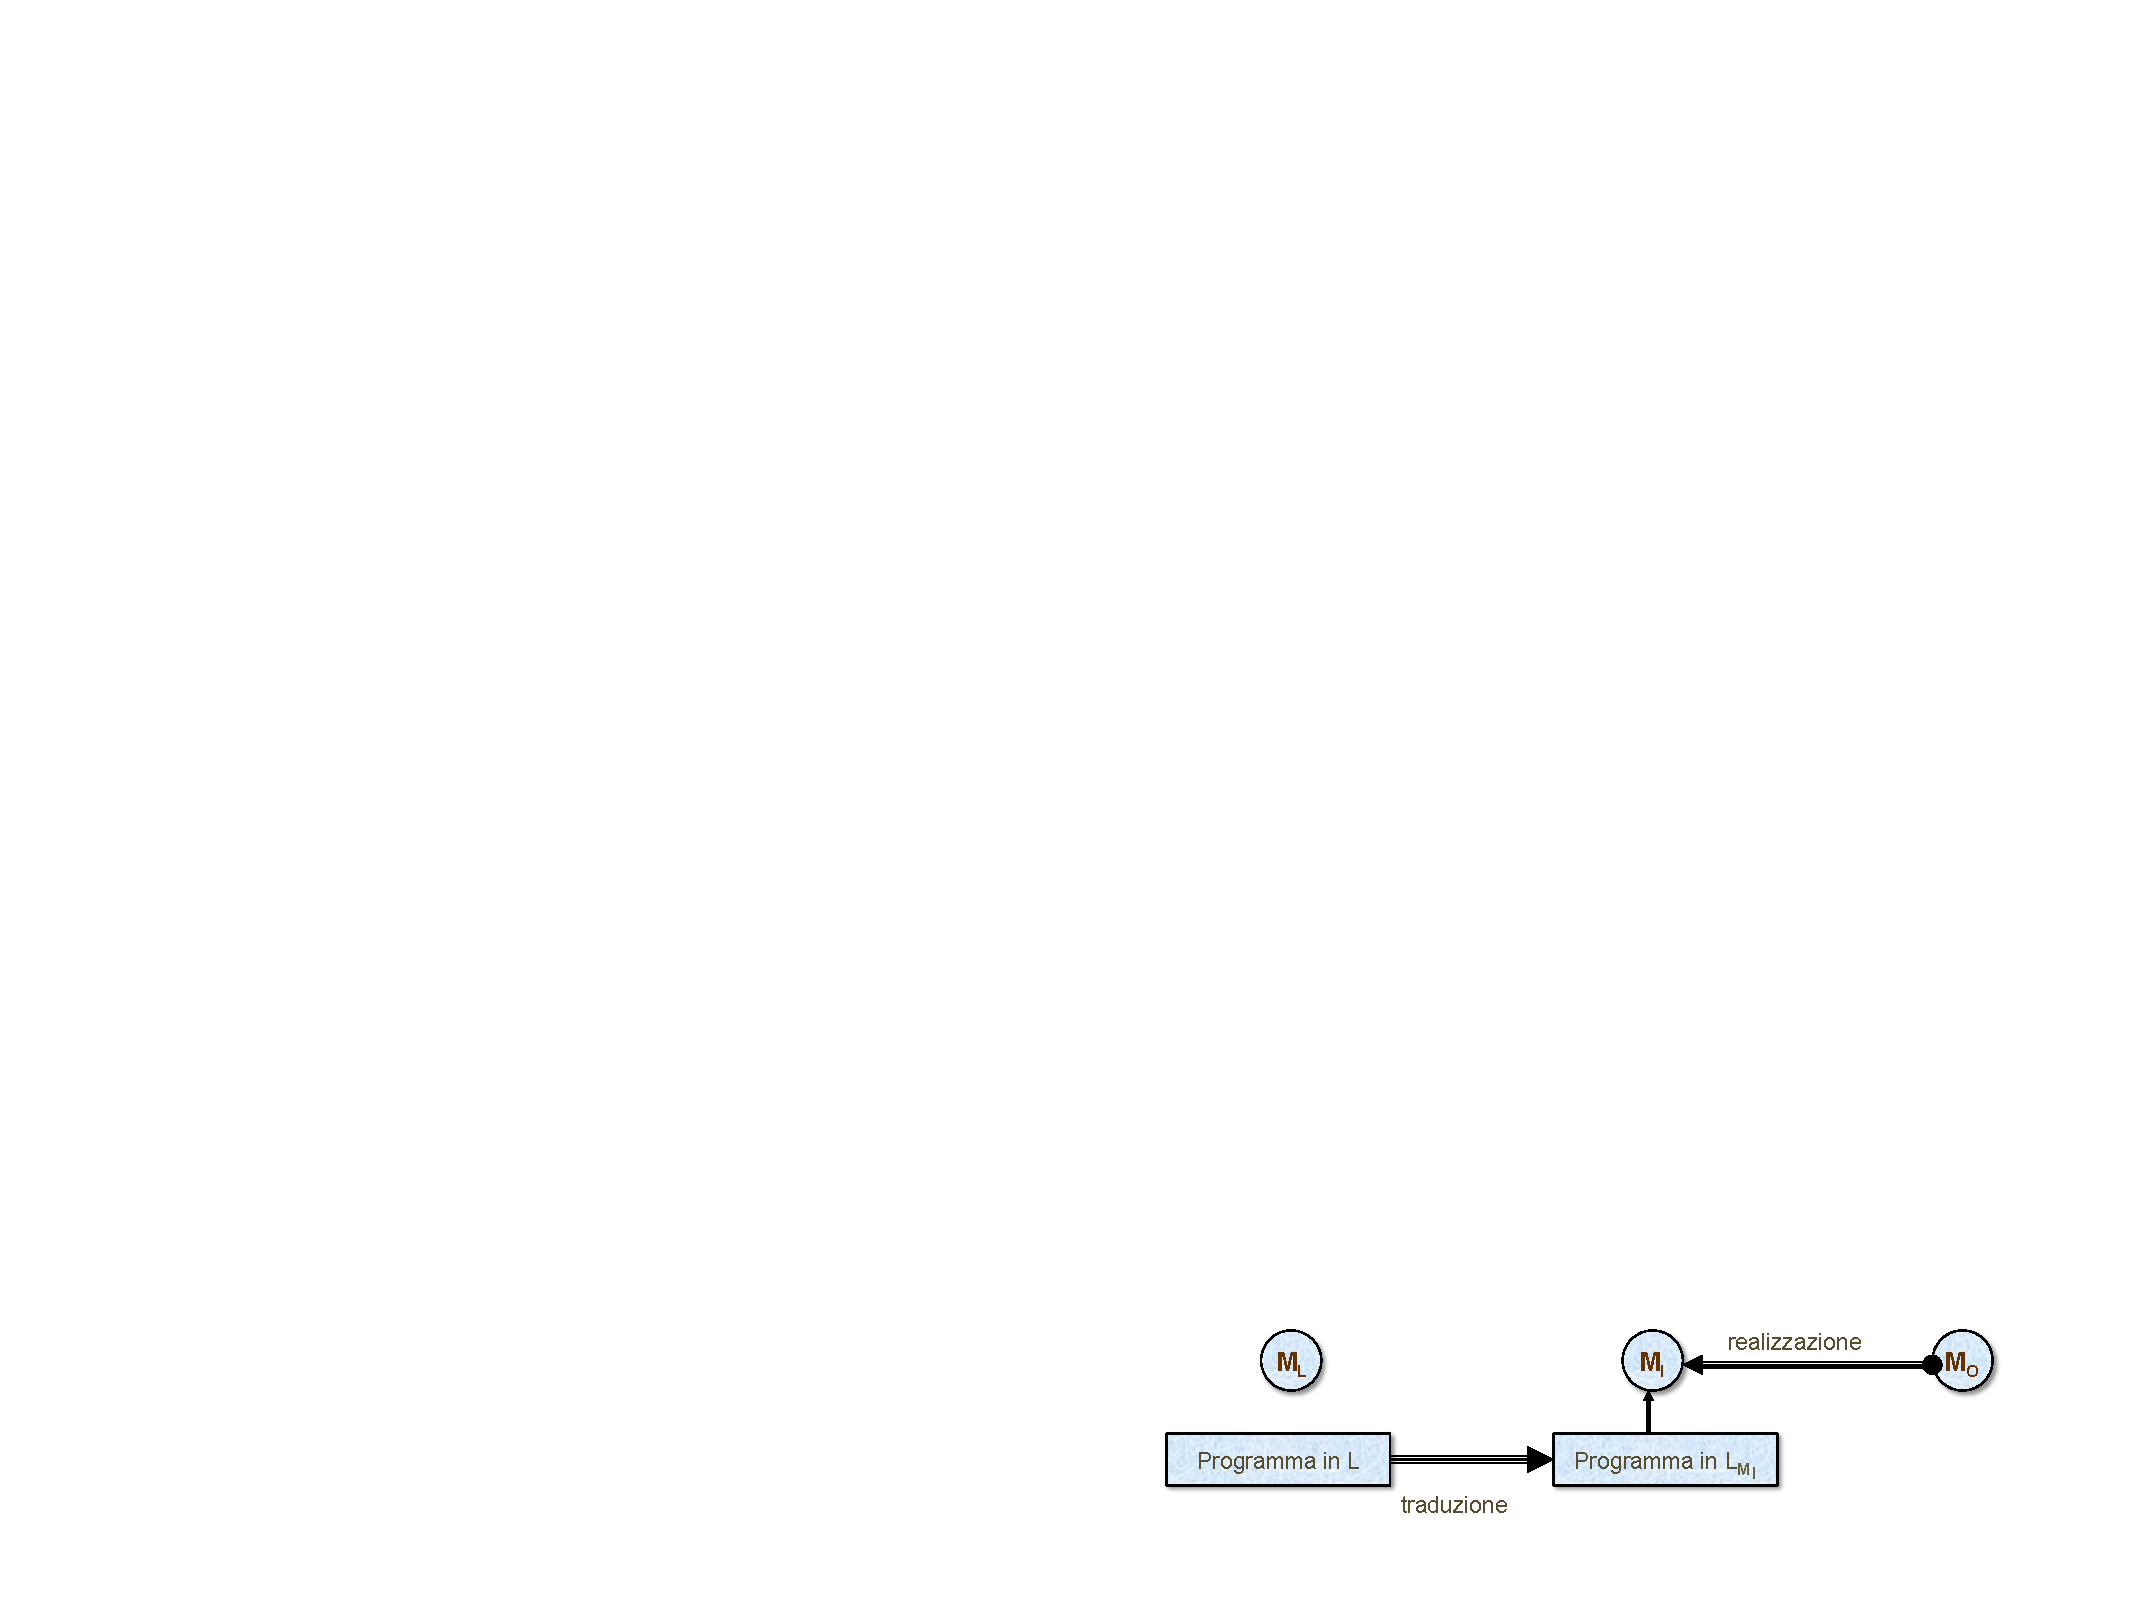
\includegraphics[width=\textwidth]{img/soluzione_ibrida_system_call.pdf}
		\caption{Soluzione ibrida con le \emph{system call}.}
	\end{figure}

	\longline

	\subsection{Sintesi}

	Nell'evoluzione dei linguaggi di programmazione, esistono fondamentalmente tre situazioni possibili:
	\begin{itemize}
		\item \textcolor{Red3}{\textbf{Interprete puro}} (paragrafo \ref{interprete}), $M_{L} = M_{I}$ (interprete per $L$ realizzato sulla macchina ospite $M_{O}$). Per esempio i linguaggi logici e funzionali, e di scripting (JS, PHP, ...)

		\item \textcolor{Red3}{\textbf{Compilatore}} (paragrafo \ref{compilatore}), macchina intermedia $M_{I}$ realizzata per estensione sulla macchina ospite $M_{O}$. Per esempio i linguaggi imperativi come C, C++, Pascal
		
		\item \textcolor{Red3}{\textbf{Implementazione mista}} (paragrafo \ref{ibrido}), traduzione dei programmi da $L$ ad un linguaggio intermedio $L_{Mi}$. I programmi $L_{Mi}$ sono poi interpretati sulla macchina ospite $M_{O}$. Per esempio, Java con il suo linguaggio intermedio Java bytecode, Pascal con il suo linguaggio intermedio P-code.
	\end{itemize}\newpage

	\section{Descrivere i linguaggi}

	Un \textbf{linguaggio di programmazione} è un linguaggio naturale, ma con alcune semplificazioni e \textbf{non ambiguo}. Quindi, per descriverli è necessario affrontare alcune tematiche:
	\begin{itemize}
		\item Grammatica, o meglio la \textcolor{Red3}{\textbf{sintassi}}: costituisce l'\textbf{insieme delle regole che consentono di costruire frasi corrette}. Viene quindi individuato l'alfabeto con cui sono costruite le frasi, le parole che compongono le frasi e infine viene eseguito un controllo della grammatica per verificare se le frasi le rispettano (il compito di verificare è assegnato al \textbf{\emph{parsing}});
		\item \textcolor{Red3}{\textbf{Semantica}}: nei linguaggi rappresenta la \textbf{relazione tra segni} (frasi legali) \textbf{e significati} (entità autonome che esistono indipendentemente dai segni utilizzati). Per esempio, la semantica di un programma può essere la funzione matematica calcolata dal programma. Solitamente la semantica viene specificata descrivendo gli effetti della sintassi su una rappresentazione astratta della macchina, chiamata \textbf{stato};
		\item \textcolor{Red3}{\textbf{Pragmatica}}: analisi delle \textbf{frasi che hanno lo stesso significato, ma possono essere utilizzate diversamente} in modo dipendente dal contesto linguistico;
		\item \textcolor{Red3}{\textbf{Implementazione}}: aspetti riguardanti la tecnica di implementazione utilizzata, i vincoli dell'architettura o della macchina, l'interfaccia del sistema operativo, gestione degli errori.\newline
		In sintesi, sono tutti gli aspetti che hanno effetto sul funzionamento del linguaggio ma che dipendono dalla macchina su cui esso viene eseguito.
	\end{itemize}\newpage

	\subsection{Sintassi}

	\subsubsection{Definizione e notazione}

	Le regole sintattiche (\textcolor{Red3}{\textbf{sintassi}}) del linguaggio specificano quali stringhe di caratteri sono legali nel linguaggio.\newline
	
	\noindent
	La terminologia linguistica utilizzata è la seguente:
	\begin{itemize}
		\item Una \textbf{parola} è una stringa di caratteri su un alfabeto;
		\item Una \textbf{frase} è una sequenza, ben formata, di parole;
		\item Una \textbf{linguaggio} è un insieme di frasi.
	\end{itemize}
	Invece, la \textbf{terminologia tecnica} utilizzata nel mondo dell'informatica è la seguente:
	\begin{itemize}
		\item Le \textbf{parole} vengono chiamate \textcolor{Red3}{\textbf{lessemi}}. Un lessema è una \textbf{parola con un significato specifico}, nella grammatica corrisponde ad un terminale. Rappresenta anche l'\textbf{unità minima sintattica}, ovvero quella a più basso livello di un linguaggio di programmazione (e.g. \textsf{begin}). \textbf{Per esempio}, in $index = 2$, sia $index$, $=$, che $2$ sono lessemi;
		\item Le \textbf{frasi} vengono chiamate \textcolor{Red3}{\textbf{\emph{token}}}. Essi corrispondono agli elementi delle categorie sintattiche del linguaggio di programmazione, e nella grammatica corrispondono alle sequenze generate dai simboli non terminali. \textbf{Per esempio}, con $index = 2$, il token è l'intera definizione;
		\item Il \textcolor{Red3}{\textbf{programma}} è una sequenza/composizione sequenziale, nella grammatica, di frasi ben formate;
		\item I linguaggi diventa il \textcolor{Red3}{\textbf{linguaggio di programmazione}}, ovvero tutti gli strumenti formali che lo definiscono.
	\end{itemize}\newpage

	\subsubsection{Descrivere la sintassi}

	Nei linguaggi di programmazione, il \textbf{linguaggio dei lessemi} è in generale sempre un linguaggio \textbf{regolare}, ovvero \textbf{riconosciuto} da un automa a stati finiti. Si definisce \textcolor{Red3}{\textbf{riconoscitore}}, uno \textbf{strumento di riconoscimento che legge in input stringhe sull'alfabeto del linguaggio e decide se la stringa appartiene o meno al linguaggio}.\newline
	
	\noindent
	Per esempio, l'analisi sintattica, la quale riconosce lessemi, di un compilatore.\newline

	\noindent
	Sia $L$ un linguaggio su un alfabeto $\Sigma$, per \textbf{costruire un riconoscitore} è necessario avere un meccanismo $R$ in grado di leggere (input) le stringhe di caratteri e dire (output) se essa appartiene oppure no al linguaggio $L$. Si ricorda, che questo è possibile perché il linguaggio è regolare.\newline

	\noindent
	Il \textbf{linguaggio dei \emph{token}}, e quindi dei programmi, è in generale un \textbf{linguaggio \emph{context-free} (CF)}, quindi viene \textbf{generato} da una grammatica CF. Si definisce \textcolor{Red3}{\textbf{generatore}}, uno \textbf{strumento che genera stringhe di un linguaggio}. Inoltre, un generatore può determinare se la sintassi di una particolare chiave è sintatticamente corretta confrontandola con la struttura del generatore (\emph{parser}).

	\longline

	\subsection{Grammatiche \emph{context-free}}

	Una \textcolor{Red3}{\textbf{grammatica libera dal contesto}} (o \emph{context-free}, CF) è una quadrupla $G = \left\langle V, T, P, S \right\rangle$, dove:
	\begin{itemize}
		\item $V$ è un insieme finito di variabili, chiamati anche simboli non terminali. Rappresenta le \textbf{categorie sintattiche}, ovvero gli \textbf{elementi della frase};
		\item $T$ è un insieme finito di simboli terminali $\left(V \cap T = \emptyset\right)$. Rappresenta il \textbf{vocabolario}, ovvero la \textbf{collezione di lessemi};
		\item $P$ è un insieme finito di produzioni; ogni produzione è della forma $A \rightarrow \alpha$, dove:
		\begin{itemize}
			\item $A \in V$ è una variabile
			\item $\alpha \in \left(V \cup T\right)$
		\end{itemize}
		Questo insieme rappresenta la \textbf{collezione di regole di formazione/composizione};
		\item $S \in V$ è una variabile speciale, chiamata simbolo iniziale. Rappresenta la \textbf{categoria delle frasi}.
	\end{itemize}
	La proprietà CF è anche uno svantaggio per i linguaggi di programmazione, infatti tali grammatiche non riescono a catturare vincoli contestuali. Per esempio, poter utilizzare una variabile se e solo se questa è stata precedentemente dichiarata/definita.\newpage

	\subsection{Notazione BNF}

	La \textcolor{Red3}{\textbf{BNF}} è un metalinguaggio, ovvero un \textbf{linguaggio usato per descrivere altri linguaggi}. Venne introdotto perché in passato accadeva che chi progettava ogni implementazione di un compilatore, dava significati diversi agli stessi costrutti. Questo si traduceva che programmi scritti in un linguaggio di programmazione, sviluppati per macchine diverse, non erano confrontabili.\newline

	\noindent
	Questa notazione è utilizzata per descrivere grammatiche CF, dove si usano intere parole come simboli terminali, i non terminali sono identificati racchiudendoli tra parentesi angolate $<>$, e per le produzioni si utilizza il simbolo $\Coloneqq$ al posto della freccia.
	\begin{equation*}
		\begin{array}{lll}
			<A> & \Coloneqq & \alpha <B> \gamma \hspace{1em} | \hspace{1em} \alpha \\
			\\
			<B> & \Coloneqq & \varepsilon \hspace{1em} | \hspace{1em} \beta_{1} \hspace{1em} | \hspace{1em} \beta_{2}
		\end{array}
	\end{equation*}
	Il suo significato è esattamente identico a quello delle grammatiche. Quindi:
	\begin{itemize}
		\item \textbf{Non terminali} sono astrazioni utilizzate per rappresentare classi di strutture sintattiche;
		\item \textbf{Terminali} sono lessemi;
		\item Ogni regola ha una parte \textbf{sinistra} contenente un \textbf{non terminale};
		\item Ogni regola ha una parte \textbf{destra} contenente una \textbf{stringa di terminali e non terminali}.
	\end{itemize}
	Esiste anche la \textcolor{Red3}{\textbf{variante EBNF}} che aggiunge la possibilità di rappresentare le \textbf{opzioni}:
	\begin{itemize}
		\item Le \textbf{parentesi quadre} $[\:]$ indicano nessuna o un'occorrenza del contenuto;
		\item Le \textbf{parentesi graffe} $\{\:\}$ indicano nessuna o più occorrenze di quanto contenuto.
		\item La \textbf{virgola} $,$ consente di esprimere più opzioni in or logico.
	\end{itemize}
	Un esempio:
	\begin{equation*}
		<A> \Coloneqq \alpha \: \left[\beta_{1}, \beta_{2}\right] \: \gamma \hspace{1em} | \hspace{1em} \alpha \: \gamma \hspace{1em} | \hspace{1em} \gamma
	\end{equation*}\newpage

	\subsection{Descrivere un semplice linguaggio imperativo}

	Un \textbf{linguaggio può essere descritto in modo informale} descrivendo quali caratteristiche inserire e il loro significato:
	\begin{itemize}
		\item Niente dichiarazioni;
		\item Solo variabili ed espressioni booleane;
		\item Assegnamento e composizione sequenziale;
		\item Comando condizionale;
		\item Comando iterativo (\emph{loop}).
	\end{itemize}
	Nonostante possa essere sufficiente per scrivere un programma corretto e interpretabile da un altro programmatore, esso \underline{non} è adeguato per costruire un compilatore o un interprete.\newline
	
	\noindent
	Per costruire un compilatore o un interprete è necessario scendere ad un livello più formale.\newline

	\noindent
	\textbf{È necessario che un linguaggio sia descritto a più livelli di astrazione ed ogni strato sia descritto da una grammatica}.

	\begin{figure}[!htp]
		\centering
		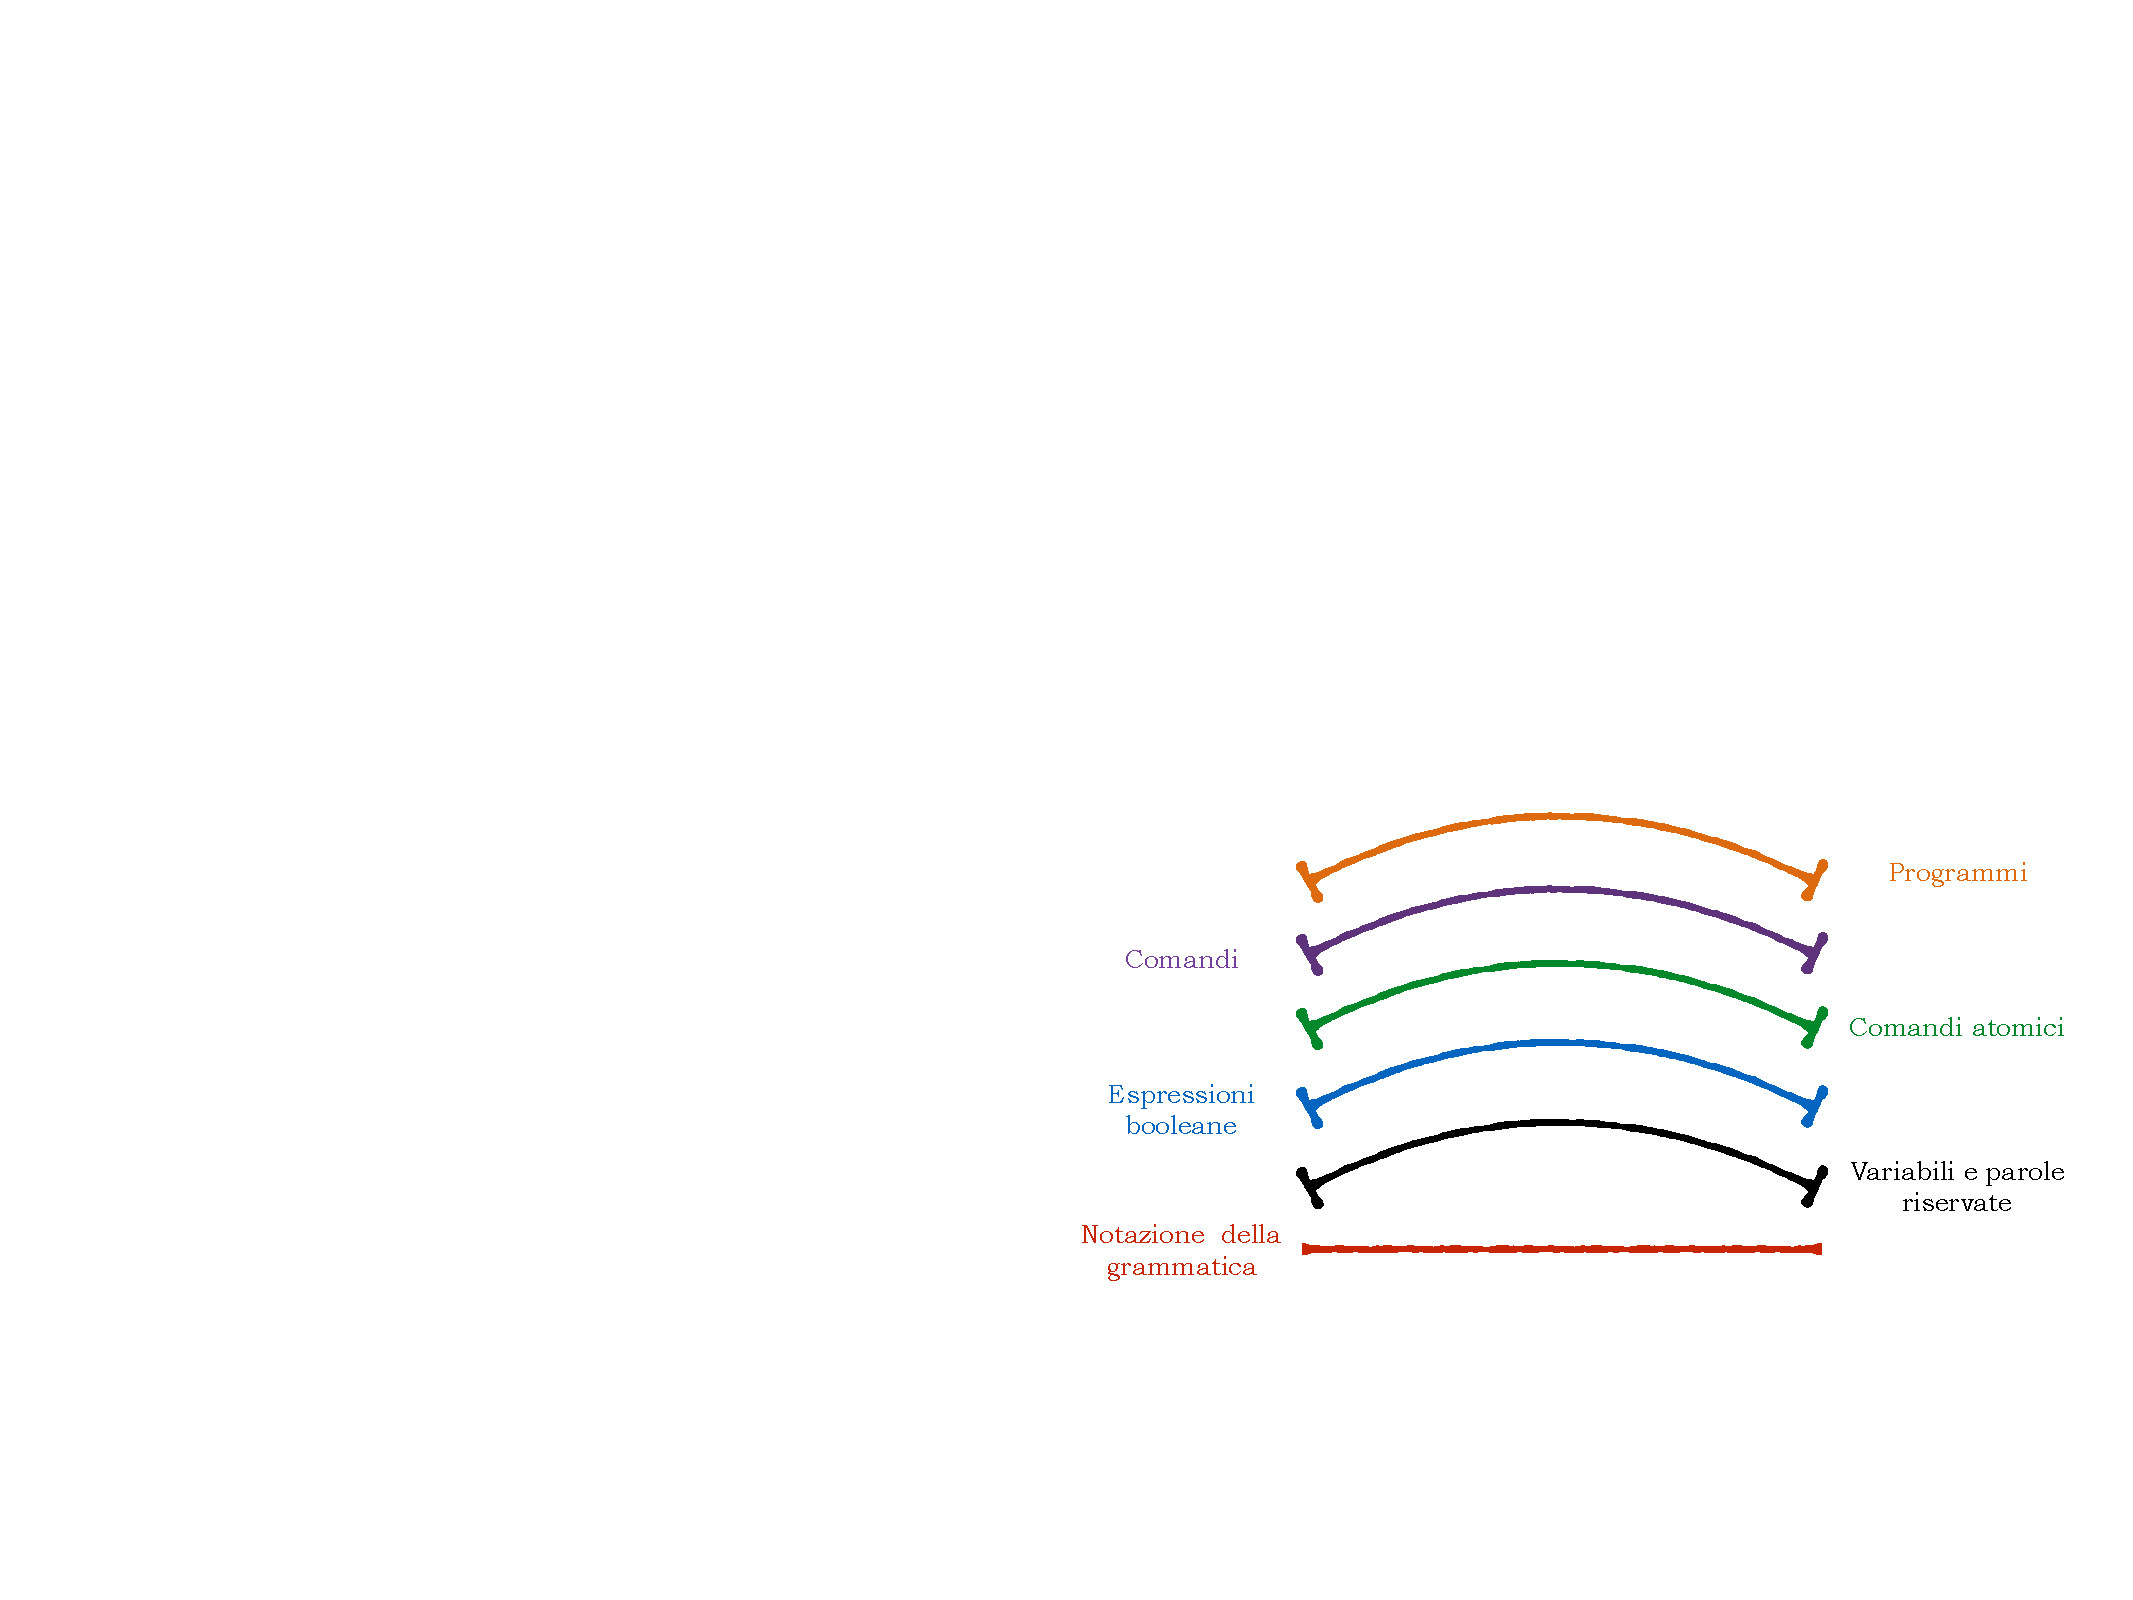
\includegraphics[width=\textwidth]{img/astrazione_linguaggi.pdf}
		\caption{Linguaggio descritto a più livelli di astrazione.}
	\end{figure}

	\noindent
	Un esempio di descrizione a più livelli:
	\begin{equation*}
		\begin{array}{lllll}
			\mathrm{<program>} 		&& S & \Coloneqq & C \\
			\\
			\mathrm{<com>}			&& C & \Coloneqq & A \hspace{1em} | \hspace{1em} C ; C \hspace{1em} | \hspace{1em} \mathrm{if} \: B \: \mathrm{then} \: C \: \mathrm{else} \: C \hspace{1em} | \hspace{1em} \mathrm{while} \: B \: \mathrm{do} \: C \\
			\\
			\mathrm{<atomic \: com>}&& A & \Coloneqq & v \Coloneq B \\
			\\
			\mathrm{<b-expr>}		&& B & \Coloneqq & \mathrm{true} \hspace{1em} | \hspace{1em} \mathrm{false} \hspace{1em} | \hspace{1em} v \hspace{1em} | \hspace{1em} \left(\mathrm{not} \: B\right) \hspace{1em} | \hspace{1em} \left(B \: \mathrm{and} \: B\right) \hspace{1em} | \hspace{1em} \left(B \: \mathrm{or} \: B\right)
		\end{array}
	\end{equation*}\newpage

	\subsection{Analisi semantica}

	Esistono dei vincoli che dipendono dal contesto. Per esempio, l'espressione:
	\begin{equation*}
		I \Coloneq R + 3
	\end{equation*}
	Potrebbe essere sintatticamente corretta ma illegale nel contesto in cui si trova. Infatti, se il linguaggio fosse fortemente \emph{tipato} e prima non ci fosse una dichiarazione di $R$ e di $I$, il comando sarebbe illegale.\newline

	\noindent
	Quindi, stringhe sintatticamente corrette per una certa grammatica sono legali sono in determinati contesti. Questo \textbf{vincolo sintattico} non può essere descritto mediante le grammatiche CF.\newline

	\noindent
	Esistono due \textbf{soluzioni}:
	\begin{itemize}
		\item Utilizzare grammatiche contestuali (CSG). Tuttavia, non esistono algoritmi lineari per il riconoscimento di stringhe generate, quindi non esistono algoritmi efficienti per effettuare il parser delle stringhe di una CSG.
		\item Utilizzare controlli \emph{ad hoc}.
	\end{itemize}
	A causa dei problemi con le grammatiche contestuali, la scelta ricade nell'utilizzare una specifica del linguaggio mediante una grammatica CF (\textbf{sintassi}) e successivamente, come parte della semantica (\textcolor{Red3}{\textbf{semantica statica}}) specificare i vincoli contestuali.\newpage

	\subsection{Semantica dinamica}

	La \textbf{semantica} ricerca esattezza e flessibilità:
	\begin{itemize}
		\item \textbf{Esattezza}: descrizione precisa e non ambigua di ogni costrutto sintatticamente corretto, per sapere cosa accadrà durante l'esecuzione
		\item \textbf{Flessibilità}: nessuna anticipazione delle scelte che devono essere demandate dall'implementazione.
	\end{itemize}
	La \textcolor{Red3}{\textbf{semantica dinamica}} risponde ad alcune problematiche, come il significato di alcuni comandi, che cosa fanno i costrutti, generatori di compilatori. Il suo \textbf{utilizzo è fondamentale poiché specifica gli effetti della sintassi sulla rappresentazione astratta della macchina}, quest'ultima chiamata \textbf{stato}.\newline
	Quindi, per ogni costrutto, va descritto il significato della sua esecuzione come trasformazione di stato. Infatti, l'astrazione della macchina nel concetto di stato consente di dare al costrutto un significato puro, indipendente dalla macchina, quindi senza restrizioni.\newline

	\noindent
	La \textcolor{Red3}{\textbf{semantica}} \textbf{attribuisce un significato ad ogni frase sintatticamente corretta}. Con \textcolor{Red3}{\textbf{significato}} \textbf{si intendono le entità autonome che esistono indipendentemente dai segni che vengono utilizzati per descriverle}.\newline

	\noindent
	Esiste un \textbf{legame forte tra sintassi e semantica}:
	\begin{itemize}
		\item La \textbf{sintassi} è utilizzato come metodo finito per rappresentare un insieme infinito di programmi, la cui sola cosa analizzabile è la struttura;
		\item La \textbf{semantica} è utilizzata come metodo finito, infatti segue la struttura della sintassi, per dare significato a tutti gli elementi dell'insieme infinito dei programmi.
	\end{itemize}\newpage

	\subsection{Induzione matematica e strutturale}

	La semantica segue la struttura della sintassi, mentre quest'ultima è definita descrivendo gli elementi base e componendo questi elementi, attraverso regole, in elementi composti. Questa forma di definizione si chiama \textcolor{Red3}{\textbf{induzione}} e più formalmente è: data un insieme $A$ ed una relazione binaria $< \subseteq A \times A$ ben fondata (senza catene discendenti infinite), se $A = Nat$ si ha \textbf{induzione matematica}; se $A = L\left(G\right)$ è un linguaggio generato da una grammatica $G$, allora si ha \textbf{induzione strutturale}.\newline

	\noindent
	Il \textcolor{Red3}{\textbf{principio di induzione strutturale}} si basa sulla seguente definizione. Per dimostrare che una proprietà è valida per tutti gli elementi di una categoria sintattica:
	\begin{enumerate}
		\item \textbf{Base induttiva}: si dimostra la proprietà per tutti gli elementi base della categoria, quelli che non hanno nessun elemento come componente;
		\item \textbf{Passo induttivo}: si dimostra la proprietà per tutti gli elementi composti assumendo che la proprietà sia verificata da tutti i loro componenti immediati.
	\end{enumerate}
	Ecco un esempio.
	\begin{proof}[\textbf{Dimostrazione induttiva}]
		Dimostrare che:
		\begin{equation*}
			\sum_{i = 1}^{n} i = \dfrac{n \left( n + 1 \right)}{2} \hspace{2em} \text{con } n \ge 1
		\end{equation*}
		La \textbf{base induttiva} è con $n$ pari ad $1$, quindi sostituendo:
		\begin{equation*}
			n = 1 \hspace{2em} \sum_{i = 1}^{1} i = 1 = \dfrac{1 \left( 1 + 1 \right)}{2}
		\end{equation*}
		Per il \textbf{passo induttivo} si suppone che sia vero per $n$ considerando dunque come passo induttivo l'equazione iniziale. Si dimostra per $n + 1$:
		\begin{equation*}
			\begin{array}{rll}
				\displaystyle\sum_{i=1}^{n+1} i & = & \dfrac{ \left(n+1\right) \left(n+2\right) }{2} \\
				\\
				\displaystyle\sum_{i=1}^{n+1} i \triangleq \underbrace{\sum_{i=1}^{n} i + \left(n+1\right)}_{\text{per definizione}} & = & \underbrace{\dfrac{n \left(n+1\right)}{2}}_{\text{ip. induttiva}} + \: n + 1 \\
				\\
				& = & \dfrac{n \left(n+1\right) + 2n + 2}{2} = \dfrac{n^{2} + n + 2n + 2}{2} \\
				\\
				& = & \dfrac{\left(n+1\right) n + \left(n+1\right) 2}{2} = \dfrac{\left(n+1\right) \left(n+2\right)}{2}
			\end{array}
		\end{equation*}
	\end{proof}\newpage

	\subsection{Un significato, tante rappresentazioni}
	
	Durante l'implementazione di un algoritmo, ci sono alcuni aspetti che un programmatore deve tenere in considerazione:
	\begin{itemize}
		\item Il \textbf{comportamento dell'I/O} è un aspetto che interessa l'\textbf{implementatore}, ovvero colui che descrive funzionalità attraverso le trasformazioni di stato della macchina.
	
		\item La funzione descritta dall'algoritmo è un aspetto che interessa il \textbf{progettista}, ovvero colui che progetta costrutti del linguaggio per consentire l'implementazione di certe funzionalità.
	
		\item Le \textbf{proprietà e invarianti} sono di interesse dello sviluppatore, ovvero colui che è focalizzato sull'utilizzo e sulla combinazione dei costrutti così di preservare invarianti o da garantire proprietà desiderate.
	\end{itemize}
	Di fatto tutte queste rappresentazioni, e i loro punti di vista, sono equivalenti, guardano solo il problema da diversi punti. Per questo motivo, nascono \textbf{diversi tipi di semantica}:
	\begin{itemize}
		\item \textbf{Semantica denotazionale}: descrive funzionalità. Studia gli effetti dell'esecuzione e cerca proprietà del programma studiando proprietà della funzione calcolata;
		
		\item \textbf{Semantica assiomatica}: descrive proprietà. Necessaria per fare deduzioni logiche, a partire da assiomi dati, su parti del programma (dimostrazioni di correttezza);
		
		\item \textbf{Semantica operazionale}: descrive trasformazioni di stato. Opera con l'obbiettivo di analizzare il processo per arrivare ad un risultato finale. In parole povere, ha l'obbiettivo di analizzare come i risultati finali vengono prodotti (implementazione di un interprete).
	\end{itemize}\newpage

	\subsubsection{Semantica denotazionale}
	
	La \textcolor{Red3}{\textbf{semantica denotazionale}} è un modello matematico dei programmi basato sulla ricorsione. È la semantica più \dquotes{astratta} con cui descrivere i programmi.\newline
	
	\noindent
	Il \textbf{processo di costruzione} della semantica denotazionale \textbf{per un linguaggio} si articola in due passaggi fondamentali:
	\begin{enumerate}
		\item Definizione di un oggetto matematico per ogni entità del linguaggio;
		
		\item Definizione di una funzione che esegue un \emph{mapping} delle istanze delle entità del linguaggio in istanze dei corrispondenti oggetti matematici.
	\end{enumerate}
	Il modello matematico utilizzato è quello delle funzioni matematiche ricorsive, ovvero un programma corrispondente ad una funzione tra stati della macchina:
	\begin{equation*}
		E: \mathrm{Prog} \longrightarrow \left( \left(\mathrm{Var} \rightarrow \mathrm{Val}\right) \longrightarrow \left(\mathrm{Var} \rightarrow \mathrm{Val}\right) \right)
	\end{equation*}
	L'equivalenza di programma si dimostra mediante equivalenza tra funzioni matematiche.\newline
	
	\noindent
	Dunque la \textbf{semantica denotazionale è un oggetto puramente matematico} che descrive gli effetti semplicemente manipolando oggetti matematici.\newline
	In particolare, vengono \textbf{analizzati gli effetti dell'esecuzione del programma}, descrivendo l'effetto dell'esecuzione di una sequenza di comandi separati da \dquotes{;} attraverso la composizione degli effetti dei singoli comandi da sinistra verso destra.\newline
	Con \textbf{effetto di ogni comando} si intende la funzione che dato uno stato produce un nuovo stato.\newline
	
	\noindent
	Il suo utilizzo è \textcolor{Green4}{\textbf{utile}} per:
	\begin{itemize}
		\item Dimostrare la correttezza dei programmi;
		\item Ragionare formalmente sui programmi;
		\item Aiutare la progettazione dei linguaggi;
		\item Generare i compilatori.s
	\end{itemize}
	Purtroppo, a causa della sua elevata complessità, risulta \textcolor{Red3}{\textbf{poco utile}} per gli utilizzatori dei linguaggi.\newpage
	
	\noindent
	Per \textcolor{Green4}{\textbf{esempio}}, si definisce la funzione di valutazione $E\exec{P}\sigma$ che valuta il programma $P$ sulla memoria $\sigma$, restituendo in output $\sigma'$ che corrisponde alla memoria $\sigma$ modificata dal programma $P$.\newline
	
	\noindent
	Il programma $P$ è formato nel seguente modo:
\begin{lstlisting}[language=C]
P:
	z := 2;
	y := z;
	y := y+1;
	z := y;\end{lstlisting}
	La semantica denotazionale consente questa rappresentazione:
	\begin{equation*}
		\begin{array}{lll}
			E\exec{P}\left(z = \bot, y = \bot\right) & = & \left(E\exec{ z \coloneq y } \circ E\exec{ y \coloneq y+1 } \circ E\exec{ y \coloneq z } \circ E\exec{ z \coloneq 2 }\right) \left[z = \bot, y = \bot\right] \\
			\\
			&=& \left(E\exec{ z \coloneq y } \left( E\exec{ y \coloneq y+1 } \left( E\exec{ y \coloneq z } \left( E\exec{ z \coloneq 2 } \right) \left[z = \bot, y = \bot\right]\right)\right)\right) \\
			\\
			&=& \left(E\exec{ z \coloneq y } \left( E\exec{ y \coloneq y+1 } \left( E\exec{ y \coloneq z } \left[z = 2, y = \bot\right]\right)\right)\right) \\
			\\
			&=& \left(E\exec{ z \coloneq y } \left( E\exec{ y \coloneq y+1 } \left[z = 2, y = 2\right]\right)\right) \\
			\\
			&=& \left(E\exec{ z \coloneq y } \left[z = 2, y = 3\right]\right) \\
			\\
			&=& \left[z = 3, y = 3\right]
		\end{array}
	\end{equation*}
	Ad ogni passo viene consumata una valutazione, la quale modifica in memoria i valori tra parentesi quadre.\newpage
	
	\subsubsection{Semantica assiomatica}
	
	La \textcolor{Red3}{\textbf{semantica assiomatica}} è un modello matematico dei programmi basato sulla logica formale, ovvero il calcolo dei predicati.\newline
	
	\noindent
	L'\textbf{obbiettivo} della semantica assiomatica è la verifica formale di programmi. Per farle, vengono utilizzati assiomi e regole di inferenza. Le \textbf{espressioni logiche} utilizzate sono chiamate \textbf{asserzioni}:
	\begin{itemize}
		\item \textbf{Precondizione}: asserzione prima di un comando che dichiara le relazioni e i vincoli validi prima dell'esecuzione del comando;
		
		\item \textbf{Postcondizione}: asserzione che segue il comando che descrive cosa vale dopo l'esecuzione;
		
		\item \textbf{\emph{Weakest precondition}}: una precondizione meno restrittiva che garantisce la post-condizione.
	\end{itemize}
	Quindi, la semantica assiomatica consente di \textbf{dimostrare proprietà parziali di correttezza}: quando lo stato iniziale rispetta la precondizione e il programma termina, allora lo stato finale soddisfa la postcondizione.\newline
	
	\noindent
	Dato che la semantica assiomatica è un sistema logico, deve \textbf{godere di due proprietà}:
	\begin{itemize}
		\item \textbf{Correttezza} (\emph{soundness}), ogni proprietà derivabile nel sistema vale per il programma;
		
		\item \textbf{Completezza}, ogni proprietà che vale per il programma è derivabile nel sistema di regole.
	\end{itemize}

	\noindent
	Per \textcolor{Green4}{\textbf{esempio}}, si definisce la notazione $\left\{P\right\}$ \emph{statement} $\left\{Q\right\}$. Questa semantica si calcola mediante un sistema di prova: si ha una tripla da verificare e si cerca di dimostrarla applicando le regole.\newline
	
	\noindent
	Il programma $P$ è formato nel seguente modo:
	\begin{lstlisting}[language=C]
		P:
		z := 2;
		y := z;
		y := y+1;
		z := y;\end{lstlisting}
	\begin{figure}[!htp]
		\centering
		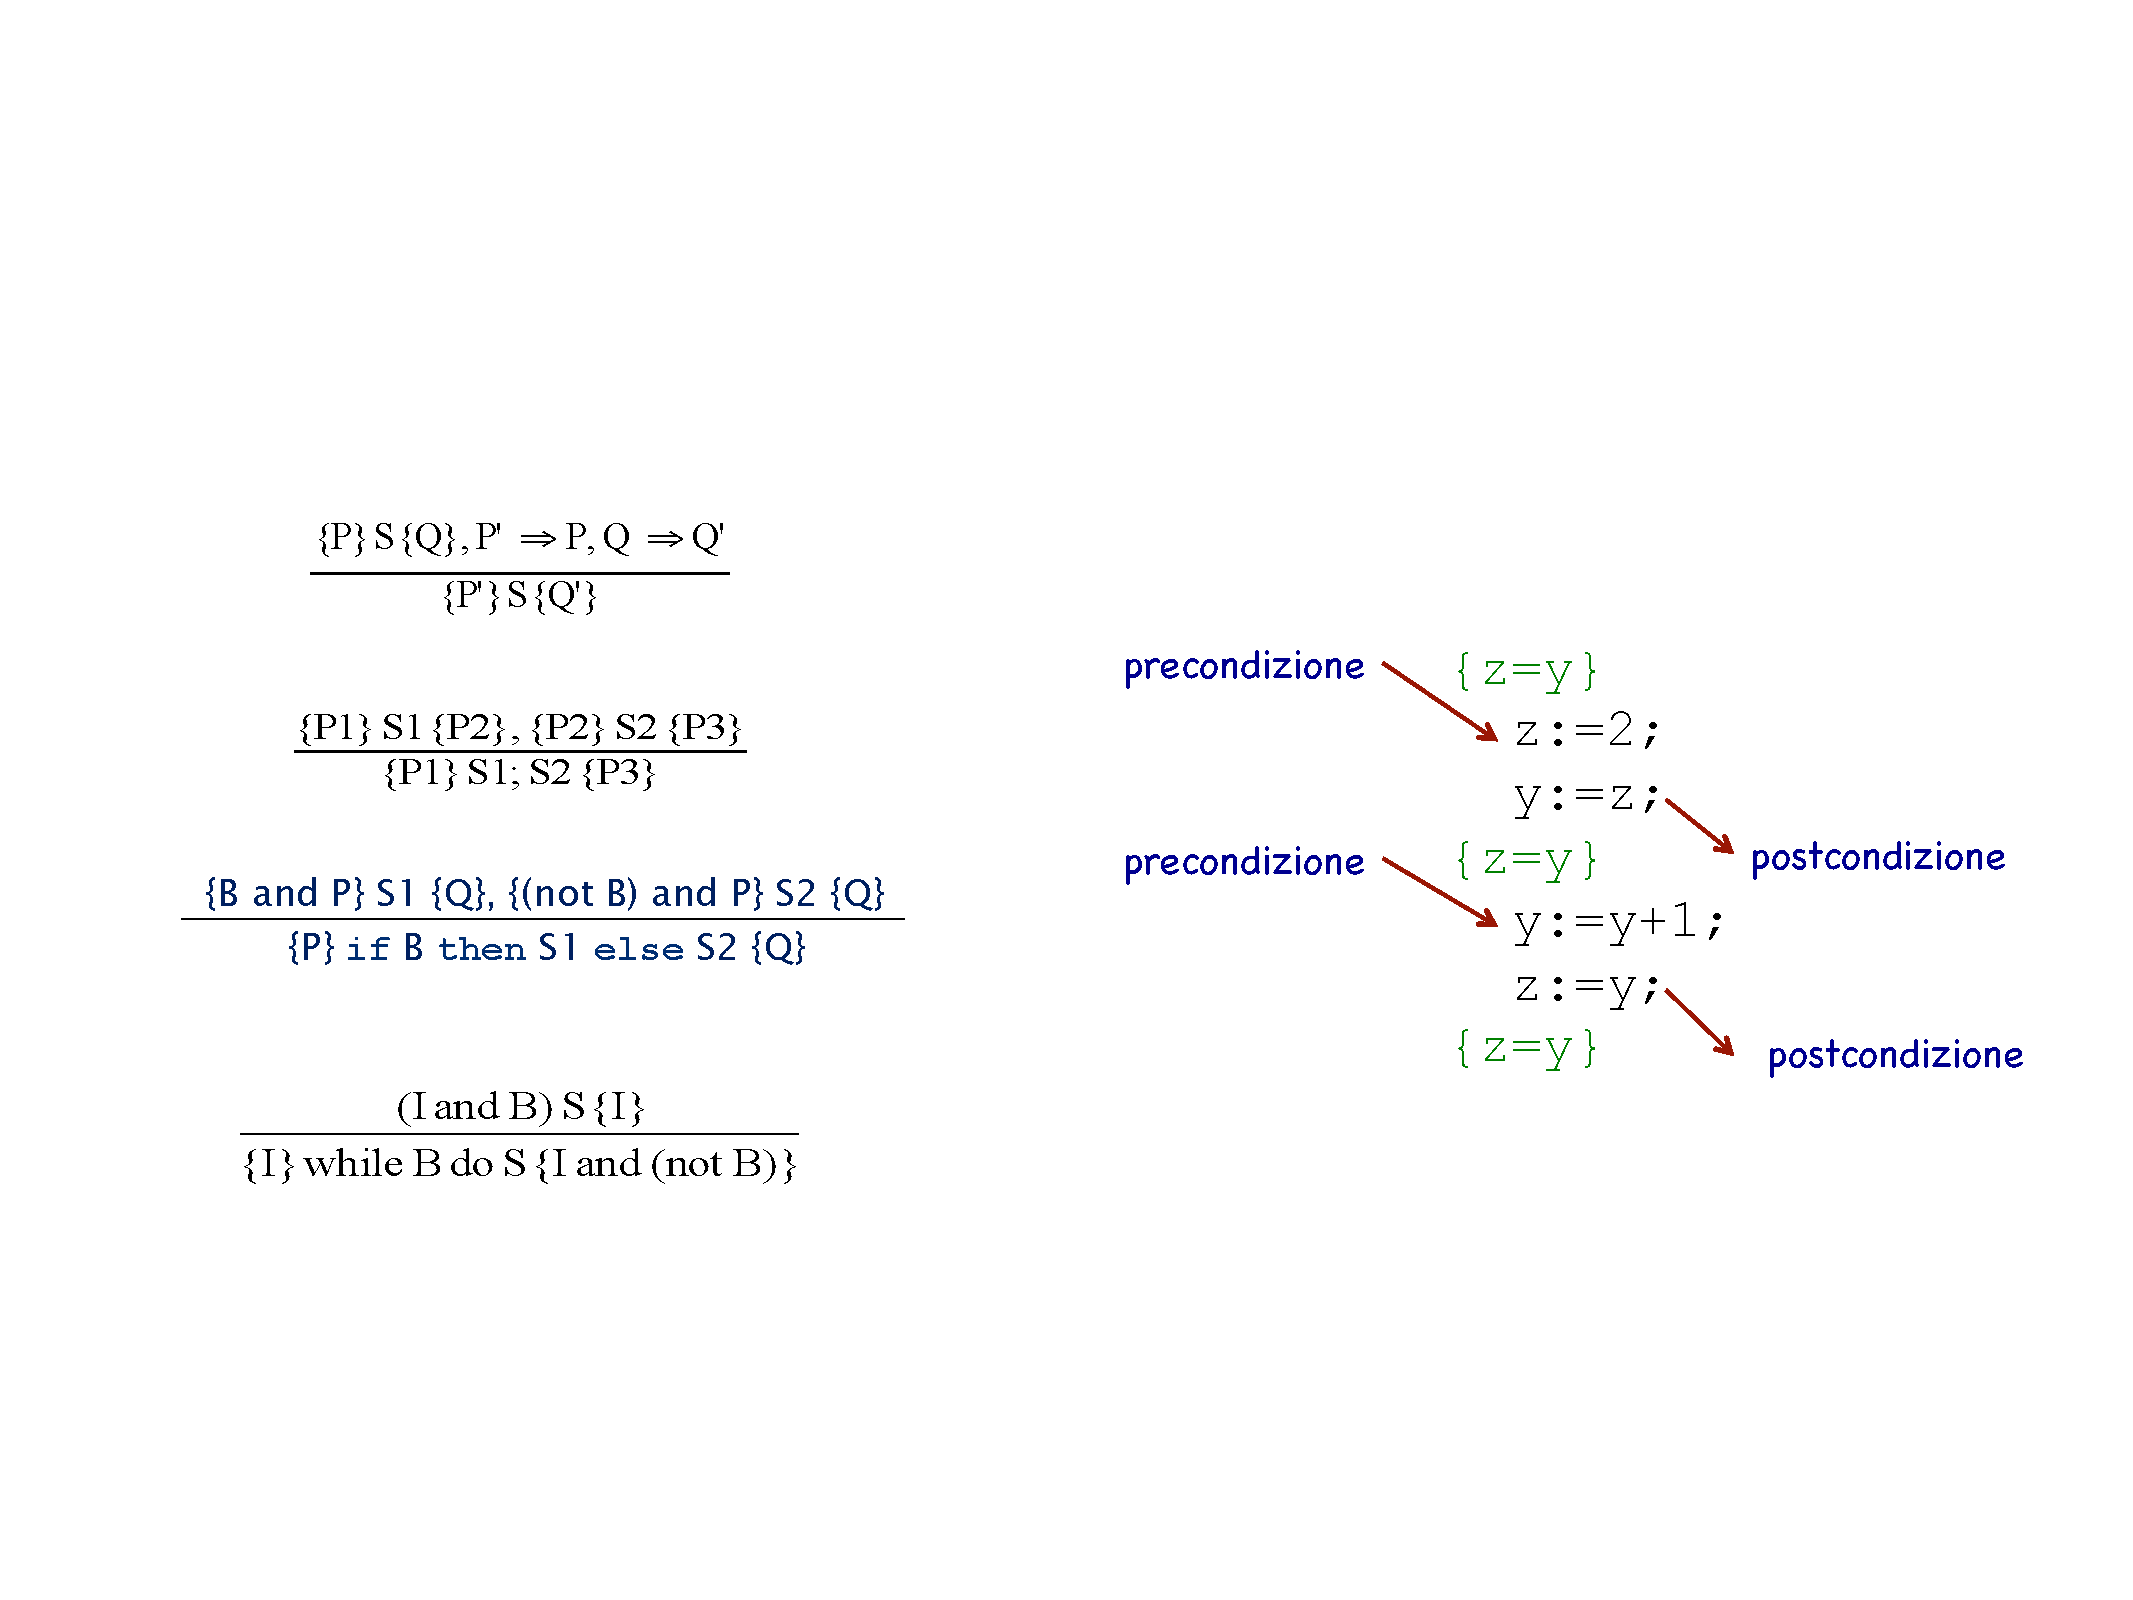
\includegraphics[width=\textwidth]{img/eg-semantica_assiomatica.pdf}
	\end{figure}\newpage

	\subsubsection{Semantica operazionale}
	
	La \textcolor{Red3}{\textbf{semantica operazionale}} è un modello matematico dei programmi basato sui sistemi di transizione.\newline
	
	\noindent
	La semantica operazionale descrive il significato del programma \textbf{eseguendo i suoi comandi su una macchina}, simulata o reale. La \textbf{trasformazione dello stato definisce il significato del comando}. Quindi, lo stato è la rappresentazione astratta della macchina.
	
	Inoltre, la semantica operazionale è necessaria per definire una macchina astratta.\newline
	
	\noindent
	Il modello matematico utilizzato è quello dei sistemi di transizione. Per \textcolor{Green4}{\textbf{esempio}}, si consideri la funzione memoria $\sigma: \mathrm{Var} \rightarrow \mathrm{Val}$ che associa valori alle variabili. Con \textbf{stato} si identifica una coppia nel programma ancora da eseguire:
	\begin{equation*}
		\mathrm{Stato} = \left\langle P,\sigma \right\rangle
	\end{equation*}
	Ad ogni passo, viene eseguita un'operazione e la configurazione o stato cambia. La chiusura transitiva descrive l'esecuzione completa.\newline
	Inoltre, questa semantica esegue i comandi separai da \dquotes{;} sequenzialmente e nell'ordine in cui compaiono da sinistra a destra.
	
	Infine, nonostante sia una delle forme più concrete di semantica, viene eseguita comunque un'astrazione di come il programma viene eseguito, quindi essa è indipendente dall'architettura.\newline
	
	\noindent
	Per \textcolor{Green4}{\textbf{esempio}}, il programma $P$ è formato nel seguente modo:
	\begin{lstlisting}[language=C]
		P:
		z := 2;
		y := z;
		y := y+1;
		z := y;\end{lstlisting}
	\begin{gather*}
		\left\langle z \coloneq 2; \hspace{1em} y \coloneq z; \hspace{1em} y \coloneq y+1; \hspace{1em} z \coloneq y, \left[z=\bot,y=\bot\right]\right\rangle \\
		\left\langle y \coloneq z; \hspace{1em} y \coloneq y+1; \hspace{1em} z \coloneq y, \left[z=2,y=\bot\right]\right\rangle \\		
		\left\langle y \coloneq y+1; \hspace{1em} z \coloneq y, \left[z=2,y=2\right]\right\rangle \\
		\left\langle z \coloneq y, \left[z=2,y=3\right]\right\rangle \\
		\left\langle \varepsilon, \left[z=3,y=3\right]\right\rangle
	\end{gather*}\newpage
	
	\subsubsection{Composizionalità}
	
	La \textcolor{Red3}{\textbf{composizionalità}} è la proprietà per cui il significato di ogni programma deve essere in funzione del significato dei costituenti immediati.\newline
	
	\noindent
	La composizionalità è una \textbf{proprietà della semantica} necessaria per caratterizzare i comportamenti e significati di sistemi che possono avere infiniti elementi.\newline
	
	\noindent
	L'\textbf{importanza} della composizionalità è dovuta alla necessità di analizzare le proprietà di un programma. Infatti, per farlo è necessario capire che cosa fa e dunque capire la semantica in ogni sua forma. L'analisi diventa molto più semplice grazie alla \textbf{modularità}, la quale è \textbf{garantita dalla composizionalità}. Quindi, anche nei software di grandi dimensioni, è possibile analizzare il codice separatamente nei suoi moduli, per poi ricomporre il risultato dell'analisi componendo i risultati ottenuti sui singoli moduli.
	
	\subsubsection{Equivalenza}
	
	L'\textcolor{Red3}{\textbf{equivalenza}} è vera quando due programmi hanno la stessa semantica.\newline
	
	\noindent
	Per capire se due programmi sono equivalenti, viene osservata la relazione tra input e output. Se la relazione è la stessa, indipendentemente da come l'algoritmo la calcola, allora sono equivalenti. Quindi, solo caratterizzando la funzionalità I/O è possibile determinare questa caratteristica.\newline
	
	\noindent
	Infine, l'equivalenza è necessaria in varie fasi di analisi:
	\begin{itemize}
		\item \textbf{Correttezza}, per dimostrare che il programma scritto calcola esattamente la funzione attesa;
		
		\item \textbf{Equivalenza di programmi}, per dimostrare che due programmi calcolano la stessa funzione;
		
		\item \textbf{Efficienza}, Dati due programmi che calcolano la stessa funzione, si vuole dimostrare quale lo fa in modo più efficiente.
	\end{itemize}\newpage
	
	\subsection{Sintassi}
	
	\subsubsection{Stato (ambiente e memoria)}
	
	Per descrivere il significato dei programmi, è necessario introdurre due entità fondamentali: ambiente e memoria.\newline
	
	\noindent
	L'\textcolor{Red3}{\textbf{ambiente}} (\textbf{\emph{environment}}) \textbf{è un insieme di legami (\emph{bindings}) tra identificatori e denotazioni}. Inoltre, l'ambiente specifica quali nomi sono usati e per quali oggetti, solitamente possono essere legati ad un tipo, ad un valore, ad una locazione. Quindi, i \emph{binding}\footnote{In breve sarebbero le API (\emph{Application Programming Interface}): \href{https://en.wikipedia.org/wiki/Language_binding}{link fonte}.} sono associati ai nomi, i quali possono essere variabili, costanti, procedure, e altro. I nomi sono solo un'entità separata dall'oggetto che denotano, infatti esso potrebbe essere usato in contesti diversi per rappresentare valori differenti.\newline
	
	\noindent
	La \textcolor{Red3}{\textbf{memoria}} (\textbf{\emph{store}}) \textbf{è un insieme di effetti sugli identificatori (causati da assegnamenti)}. Essa è una mappa che solitamente rappresenta la storia, cioè l'evoluzione, delle variazioni dei valori associati agli identificatori. In altre parole, fornisce un \emph{binding} tra locazione e valore.\newline
	Si ricorda, che la memoria è fortemente legato all'approccio imperativo, infatti i linguaggi funzionali pure non ne hanno bisogno dato che non gestiscono variabili che cambiano durante l'esecuzione del programma.
	
	\longline
	
	\subsubsection{Categorie sintattiche}
	
	Le \textcolor{Red3}{\textbf{categorie sintattiche}} \textbf{sono la classificazione dei costrutti in funzione del loro significato atteso, ovvero della classe di effetti che ha la loro esecuzione causa.}\newline
	Quindi, esse sono classi che rappresentano un diverso tipo di significato, effetto, esecuzione di un programma.\newline
	
	\noindent
	Le categorie sintattiche si distinguono in: \textbf{espressioni}, \textbf{comandi} e \textbf{dichiarazioni}. Formalmente, le categorie sono i simboli non terminali della grammatica classificati in funzione di cosa modificano dello stato e come lo modificano.\newpage
	
	\subsubsection{Espressioni}
	
	Le \textcolor{Red3}{\textbf{espressioni}} \textbf{nascono dalla necessità di avere una categoria sintattica che consenta di rappresentare e denotare i valori}. Esse possono essere espresse con dei vincoli, per esempio il tipo.\newline
	
	\noindent
	Nonostante le espressioni denotino i valori, esse \textbf{non sono locazioni di memoria}. Quest'ultime sono legati all'architettura (struttura) di una macchina, mentre le espressioni fanno riferimento allo specifico linguaggio di programmazione.\newline
	
	\noindent
	Due espressioni sono considerate \textcolor{Red3}{\textbf{equivalenti}} \textbf{se vengono valutate nello stesso valore in tutti gli stati di computazione. Anche eventuali \emph{side-effect} devono essere gli stessi}.
	
	Infatti, due espressioni possono essere diverse ma essere valutate nello stesso valore. Per \textcolor{Green4}{\textbf{esempio}}, l'espressione logica \textsf{not(a and b)} è logicamente (semanticamente) equivalente ad \textsf{(not a) or (not b)} ma sono sintatticamente diverse.
	
	\longline
	
	\subsubsection{Dichiarazioni}
	
	Le \textcolor{Red3}{\textbf{dichiarazioni}} \textbf{sono la categoria sintattica che consente la creazione o la modifica dei legami associati agli identificatori, ovvero gli ambienti}.\newline
	
	\noindent
	Esse nascono con l'obbiettivo di utilizzare i valori. Per farlo, è stato necessario creare, utilizzare e modificare \textbf{legami} tra nomi e valori.
	
	Inoltre, gli le modifiche agli ambienti sono trasformazioni \textbf{reversibili}, ovvero che le trasformazioni hanno valenza esclusivamente all'interno del raggio d'azione (\emph{scope}) attuale dell'identificatore. In altre parole, i linguaggi di programmazione delimitano la validità di un ambiente. Più precisamente con \textbf{reversibili si intende} che una volta terminata la validità di un ambiente, le modifiche verranno annullate.\newline
	
	\noindent
	Due dichiarazioni sono \textcolor{Red3}{\textbf{equivalenti}} \textbf{se producono lo stesso ambiente e la stessa memoria in caso di \emph{side-effect} in tutti gli stati di computazione}.\newline
	A causa del \emph{side-effect} è necessario che l'equivalenza richieda che due dichiarazioni generino le stesse identiche modifiche a tutto lo stato di computazione.
	
	\longline
	
	\subsubsection{Comandi}
	
	I \textcolor{Red3}{\textbf{comandi}} \textbf{sono richieste di modifica dello stato di computazione, ed in particolare della memoria}.\newline
	
	\noindent
	Le trasformazioni sono \textbf{irreversibili}, ovvero sono definite nell'esecuzione del programma. Quindi, per annullarle è necessario eseguire altri comandi e altre trasformazioni che consentono di tornare alla stessa memoria iniziale. Quindi, i comandi non sono altro che funzioni di trasformazione e devono essere \textbf{eseguiti} per poter attuare la corrispondente trasformazione (irreversibile) della memoria.
	
	Due comandi sono \textcolor{Red3}{\textbf{equivalenti}} \textbf{se per ogni stato (memoria) in input producono lo stesso stato (memoria) in output}.\newpage
	
	\subsection{Semantica operazionale: sistemi di transizione}
	
	I \textcolor{Red3}{\textbf{sistemi di transizione}} \textbf{sono strumenti astratti mirati a specificare senza ambiguità e senza dipendenza dalla macchina, cosa fa un linguaggio}. Le sue caratteristiche principali sono:
	\begin{itemize}
		\item Matematicamente precisi;

		\item Molto concisi;

		\item Metodo di specifica generale che consente l'astrazione;

		\item Specificano cosa viene calcolato per induzione sulla struttura sintattica del linguaggio.
	\end{itemize}
	Inoltre, sfruttando la definizione induttiva del linguaggio, consentono di definire il significato mediante induzione sull'\emph{abstract syntax tree}. Quindi, viene \textbf{usata l'induzione strutturale matematica per ragion sui programmi}.\newline
	
	\noindent
	Formalmente: \textbf{un \textcolor{Red3}{sistema di transizione} è una struttura $\left(\Gamma, \rightarrow\right)$, dove $\Gamma$ è un insieme di elementi $\gamma$ chiamati configurazioni e la relazione binaria $\rightarrow \subseteq \Gamma \times \Gamma$ è chiamata relazione di transizione. Se $\Gamma_{T} \subseteq \Gamma$ è un insieme di configurazioni terminali, il sistema è detto terminale.}
\end{document}